% Usage: knitr slide


\chapter{Simple and Multiple Regression Models}
{\larger\textbf{Background}}\sound{reg-1}

Regression models are used for
\bi
\item hypothesis testing
\item estimation
\item prediction
\item increasing power and precision for assessing the effect of one
  variable by adjusting for other variables that partially explain the outcome
  variable $Y$
\item confounder adjustment---getting adjusted estimates of effects
\item checking that existing summary scores (e.g., BMI) adequately
  summarize their component variables
  \bi
  \item fit a model with log height and log weight and see if ratio of
    coefficients is -2
  \ei
\item determining whether change, average, or most recent measurement
  should be emphasized
  \bi
  \item fit a model containing body weight measured 1y ago and at time
    of treatment initiation
  \item if simple change score is an adequate summary of the two
    weights, the ratio of their coefficients will be about -1
  \item if most recent weight is all-important, coefficient for weight
    1y ago will be very small
  \ei
\item developing new summary scores guided by predicting outcomes
\ei

{\larger\textbf{Example}}
\bi
\item Observational study of patients receiving treatments A and B
\item Females are more likely to receive treatment B $\rightarrow$
  need to adjust for sex
\item Regression approach: fit a model with covariates (predictors)
  treatment and sex; treatment effect is adjusted for sex
\item Stratification approach: for males estimate the B-A difference
  and do likewise for females\\Average of the two differences is
  adjusted for sex
\ei

Now instead of sex being the relevant adjustment variable suppose it
is age, and older patients tend to get treatment B
\bi
\item Regression approach: fit a model with treatment and
  age\\Treatment effect attempts to estimate the B-A difference at any
  chosen (fixed; conditioned on) age
\item Stratification approach:
  \bi
  \item divide age into quintiles
  \item within each quintile compute the B-A difference
  \item average these differences to get an almost age-adjusted
    treatment effect
  \item problem with residual heterogeneity of age within quintiles,
    especially at outer quintiles which are wider
  \ei
\item Matching approach:
  \bi
  \item for each patient on A find a patient on B within 2y of same age
  \item if no match exists discard the A patient
  \item don't use the same B patient again
  \item discard B patients who were not needed to match an A
  \item do a matched pairs analysis, e.g. paired $t$-test
  \item sample size is reduced $\rightarrow \downarrow$ power
  \ei
\ei

\section{Stratification vs.\ Matching vs.\ Regression}%
\movie{https://youtu.be/IiJ6pMs2BiA}\disc{reg-alt}
\bi
\item Some ways to hold one variable $x_1$ constant when estimating the
  effect of another variable $x_2$ (\emph{covariable adjustment}):
  \bi
  \item experimental manipulation of $x_1$
  \item stratify the data on $x_1$ and for each stratum analyze the
    relationship between $x_2$ and $Y$
  \item form matched sets of observations on the basis of $x_1$ and
    use a statistical method applicable to matched data
  \item use a regression model to estimate the joint effects $x_1$ and
    $x_2$ have on $Y$; the estimate of the $x_2$ effect in the context
    of this model is essentially the $x_2$ relationship on $Y'$ where
    $Y'$ is $Y$ after the $x_1$ effect is subtracted from it
  \ei
\item Stratification and matching are not effective when $x_1$ is
  continuous are there are many $x$'s to hold constant
\item Matching may be useful \emph{before} data acquisition is
  complete or when sample is too small to allow for regression
  adjustment for $>1$ variable
\item Matching after the study is completed usually results in
  discarding a large number of observations that would have been
  excellent matches
\item Methods that discard information lose power and precision, and
  the observations discarded are arbitrary, damaging the study's
  reproducibility
\item Most matching methods depend on the row order of observations,
  again putting reproducibility into question
\item There is no principled unique statistical approach to analysis
  of matched data
\item All this points to many advantages of regression adjustment
\ei


Stratification and matching can be used to adjust for a small set of
variables when assessing the association between a target variable and
the outcome.  Neither stratification nor matching are satisfactory
when there are many adjustment variables or any of them are
continuous.  Crude stratification is often used in randomized trials
to ensure that randomization stays balanced within subsets of subjects
(e.g., males/females, clinical sites).  Matching is an effective way
to save resources \textbf{before} a study is done.  For example, with
a rare outcome one might sample all the cases and only twice as many
controls as cases, matching controls to cases on age within a small
tolerance such as 2 years.  But once data are collected, matching is
arbitrary, ineffective, and wasteful, and there are no principled
unique statistical methods for analyzing matched data.  For example if
one wants to adjust for age via matching, consider these data:
\begin{center}\begin{tabular}{rl} \hline
Group & Ages \\ \hline
\textbf{E}xposed   & 30 35 40 42 \\
\textbf{U}nexposed & 29 42 41 42 \\ \hline
\end{tabular}\end{center}
The matched sets may be constructed as follows:
\begin{center}\begin{tabular}{rl} \hline
Set & Data \\ \hline
1 & E30 U29 \\
2 & E40 U41 \\
3 & E42 U42a \\ \hline
\end{tabular}\end{center}
U42a refers to the first 42 year old in the unexposed group.  There is no match for E35.  U42b was not used even though she was perfect match for E42.
\be
\item Matching failed to interpolate for age 35; entire analysis must be declared as conditional on age not in the interval $[36,39]$
\item $n \downarrow$ by discarding observations that are easy to match (when the observations they are easily matched to were already matched)
\item Majority of matching algorithms are dependent on the row order of the dataset being analyzed so reproducibility is in question
\ee
These problems combine to make post-sample-collection matching unsatisfactory from a scientific standpoint\footnote{Any method that discards already available information should be thought of as unscientific.}.

\href{http://www.stat.columbia.edu/~gelman/arm/chap10.pdf}{Gelman} has
a nice chapter on matching.

\section{Purposes of Statistical Models}\rms{1.1}\disc{reg-purpose}

\quoteit{Statisticians, like artists, have the bad habit of falling in
  love with their models.}{George E.\ P.\ Box}

\bigskip

\quoteit{Most folk behave and thoughtlessly believe that the objective of
analysis with statistical tools is to find / identify features in the
data---period.\\

They assume and have too much faith that (1) the data effectively
reflect nature and not noise, and (2) that statistical tools can
`auto-magically' divine causal relations.\\

They do not acknowledge that the objective of analysis should be to
find interesting features of nature (which to the extent that they
indicate causal effects will be reproducible), represent them well,
and use these features to make reliable decisions about future
cases/situations.\\

Too often the $p$-value 'satisfices', for the intent of the latter.\\

I also think that hypothesis testing and effect estimation are really
forms of ersatz prediction---ways of identifying and singling out a
factor that allows them to make prediction in a simplistic manner
(again satisficing for cognitive ease). Therefore full, well
formulated prediction modeling is to be preferred to achieve this
unacknowledged goal on these grounds.}{Drew Levy\\Genentech\\March 2015}\\

\bi
\item Hypothesis testing
 \bi
 \item Test for no association (correlation) of a predictor
  (independent variable) and a response or dependent variable
  (unadjusted test) or test for no association of predictor and
  response after adjusting for the effects of other predictors
 \ei
\item Estimation
\bi
 \item Estimate the shape and magnitude of the relationship between a
  single predictor (independent) variable and a response (dependent) variable
 \item Estimate the effect on the response variable of changing a
  predictor from one value to another
 \ei
\item Prediction
 \bi
 \item Predicting response tendencies, e.g., long-term average response
  as a function of predictors
 \item Predicting responses of individual subjects
 \ei
\ei

\section{Advantages of Modeling}\disc{reg-advantage}
Even when only testing $H_{0}$ a model based approach has advantages:
\bi
\item   Permutation and rank tests not as useful for estimation
\item   Cannot readily be extended to cluster sampling or repeated measurements
\item   Models generalize tests
    \bi
    \item   2-sample $t$-test, ANOVA \ra \\ multiple linear regression
    \item   Wilcoxon, Kruskal-Wallis, Spearman \ra \\ proportional odds
            ordinal logistic model
    \item   log-rank \ra Cox
    \ei
\item   Models not only allow for multiplicity adjustment but for
        shrinkage of estimates
    \bi
    \item   Statisticians comfortable with $P$-value adjustment
            but fail to recognize that the difference between the most
            different treatments is badly biased
    \ei
\ei
Statistical estimation is usually model-based
\bi
\item   Relative effect of increasing cholesterol from 200 to 250
        mg/dl on hazard of death, holding other risk factors constant
\item   Adjustment depends on how other risk factors relate to outcome
\item Usually interested in adjusted (partial) effects, not unadjusted
  (marginal or crude) effects
\ei

\section{Nonparametric Regression}\rms{2.4.7} \abd{17.8}
\disc{reg-nonpar}
\bi
\item Estimate tendency (mean or median) of $Y$ as a function of $X$
\item Few assumptions
\item Especially handy when there is a single $X$
\item Plotted trend line may be the final result of the analysis
\item Simplest smoother: moving average \\
\begin{center}\begin{tabular}{rrrrrr} \hline
$X$: & 1 & 2 & 3 & 5 & 8 \\
$Y$: & 2.1 & 3.8 & 5.7 & 11.1 & 17.2 \\ \hline
\end{tabular}\end{center}
\ipacue\beqa
\hat{E}(Y | X=2) &=& \frac{2.1+3.8+5.7}{3} \\
\hat{E}(Y | X=\frac{2+3+5}{3}) &=& \frac{3.8+5.7+11.1}{3}
\eeqa
 \bi
 \item overlap OK
 \item problem in estimating $E(Y)$ at outer $X$-values
 \item estimates very sensitive to bin width
 \ei
\item Moving linear regression far superior to moving avg.\ (moving
  flat line)
\item  Cleveland's moving linear regression smoother {\em
  loess} (locally weighted least squares) is the most popular
  smoother
\item  Example: differential diagnosis of acute bacterial meningitis
  vs.\ viral meningitis
\ei
\begin{Schunk}
\begin{Sinput}
require(Hmisc)
getHdata(abm)   # Loads data frame ABM (note case)
with(ABM, {
  glratio <- gl / bloodgl
  tpolys <- polys * whites / 100
  plsmo(tpolys, glratio, xlab='Total Polymorphs in CSF',
       ylab='CSF/Blood Glucose Ratio',    # Fig. (*\ref{fig:reg-glratio}*)
       xlim=quantile(tpolys,  c(.05,.95), na.rm=TRUE),
       ylim=quantile(glratio, c(.05,.95), na.rm=TRUE))
 scat1d(tpolys); scat1d(glratio, side=4) })
\end{Sinput}
\begin{figure}[htbp]

\centerline{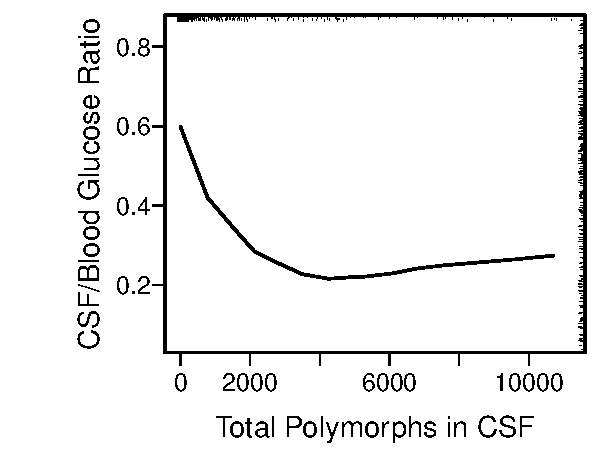
\includegraphics[width=\maxwidth]{reg-glratio-1} }

\caption[\co{loess} nonparametric smoother for glucose ratio]{\co{loess} nonparametric smoother relating CSF:blood glucose ratio to total CSF polymorph count in patients with either bacterial or viral meningitis.  Rug plot on axes plots indicate raw data values.}\label{fig:reg-glratio}
\end{figure}
\end{Schunk}
\begin{Schunk}
\begin{Sinput}
with(ABM, {
  plsmo(age, abm, 'supsmu', bass=7,     # Fig. (*\ref{fig:reg-age-abm}*)
        xlab='Age at Admission, Years',
        ylab='Proportion Bacterial Meningitis')
  scat1d(age) })
\end{Sinput}
\begin{figure}[htbp]

\centerline{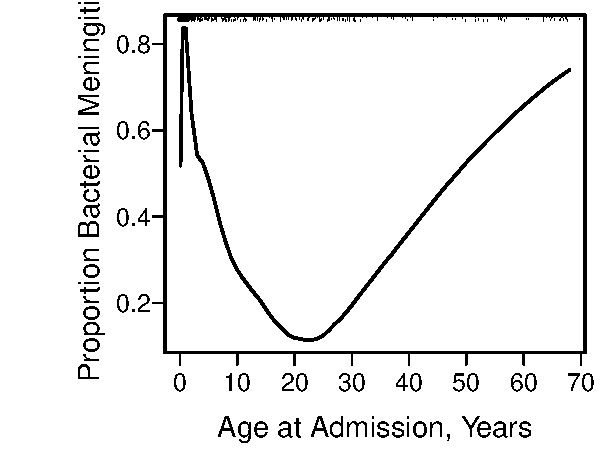
\includegraphics[width=\maxwidth]{reg-age-abm-1} }

\caption[Example of super smoother]{``Super smoother'' relating age to the probability of bacterial meningitis given a patient has bacterial or viral meningitis, with a rug plot showing the age distribution.}\label{fig:reg-age-abm}
\end{figure}
\end{Schunk}
\clearpage

\def\apacue{1}
\section{Simple Linear Regression}%
\ros{11.1-6}\abd{17-17.7,17.10-1}\sound{reg-2}\disc{reg-simple}
\subsection{Notation}
\bi
\item $y$ : random variable representing response variable
\item $x$ : random variable representing independent variable (subject
  descriptor, predictor, covariable)
  \bi
  \item conditioned upon
  \item treating as constants, measured without error
  \ei
\item What does conditioning mean?
  \bi
  \item holding constant
  \item subsetting on
  \item slicing scatterplot vertically
  \ei
\begin{Schunk}
\begin{Sinput}
n <- 100
set.seed(13)
x <- round(rnorm(n, .5, .25), 1)
y <- x + rnorm(n, 0, .1)
r <- c(-.2, 1.2)
plot(x, y, axes=FALSE, xlim=r, ylim=r, xlab=expression(x), ylab=expression(y))
axis(1, at=r, labels=FALSE)     # Fig. (*\ref{fig:reg-simple-linear-reg}*)
axis(2, at=r, labels=FALSE)
abline(a=0,b=1)
histSpike(y, side=2, add=TRUE)
abline(v=.6, lty=2)
\end{Sinput}
\begin{figure}[htbp]

\centerline{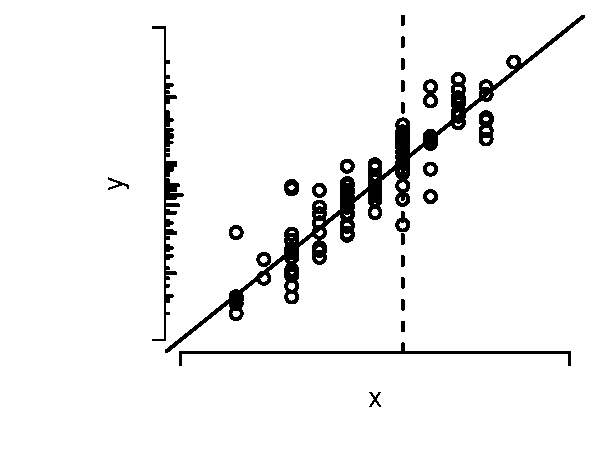
\includegraphics[width=\maxwidth]{reg-simple-linear-reg-1} }

\caption[Sample of $n=100$ points with a linear regression line]{Data from a sample of $n=100$ points along with population linear regression line.  The $x$ variable is discrete.  The conditional distribution of $y | x$ can be thought of as a vertical slice at $x$.  The unconditional distribution of $y$ is shown on the $y$-axis.  To envision the conditional normal distributions assumed for the underlying population, think of a bell-shaped curve coming out of the page, with its base along one of the vertical lines of points.  The equal variance assumption dictates that the series of Gaussian curves for all the different $x$s have equal variances.}\label{fig:reg-simple-linear-reg}
\end{figure}
\end{Schunk}
\item $E(y|x)$ : population expected value or long-run average of $y$
  conditioned on the value of $x$ \\
  Example: population average blood pressure for a 30-year old
\item $\alpha$ : $y$-intercept
\item $\beta$ : slope of $y$ on $x$ ($\frac{\Delta y}{\Delta x}$)
\ei
Simple linear regression is used when
\bi
\item Only two variables are of interest
\item One variable is a response and one a predictor
\item No adjustment is needed for confounding or other between-subject
   variation
\item The investigator is interested in assessing the strength of the
  relationship between $x$ and $y$ in real data units, or in
  predicting $y$ from $x$
\item A linear relationship is assumed (why assume this? why not use
  nonparametric regression?)
\item Not when one only needs to test for association (use Spearman's
  $\rho$ rank correlation) or estimate a correlation index
\ei
\clearpage

\subsection{Two Ways of Stating the Model}\sound{reg-3}
\bi
\item $E(y|x) = \alpha + \beta x$
\item $y = \alpha + \beta x + e$ \\
  $e$ is a random error (residual) representing variation between
  subjects in $y$ even if $x$ is constant, e.g. variation in
  blood pressure for patients of the same age
\ei
\subsection{Assumptions, If Inference Needed}
\bi
\item Conditional on $x$, $y$ is normal with mean $\alpha + \beta x$
  and constant variance $\sigma^2$, \textbf{or:}
\item $e$ is normal with mean 0 and constant variance $\sigma^2$
\item $E(y|x) = E(\alpha + \beta x + e) = \alpha + \beta x + E(e)$, \\
  $E(e) = 0$.
\item Observations are independent
\ei
\subsection{How Can $\alpha$ and $\beta$ be Estimated?}
\bi
\item Need a criterion for what are good estimates
\item \textbf{One} criterion is to choose values of the two parameters
  that minimize the sum of squared errors in predicting individual
  subject responses
\item Let $a, b$ be guesses for $\alpha, \beta$
\item Sample of size $n: (x_{1}, y_{1}), (x_{2}, y_{2}), \ldots,
  (x_{n},y_{n})$
\item $SSE = \sum_{i=1}^{n} (y_{i} - a - b x_{i})^2$
\item Values that minimize $SSE$ are \emph{least squares estimates}
\item These are obtained from

\ipacue\beqa
L_{xx} = \sum(x_{i}-\bar{x})^2 & L_{xy} = \sum(x_{i}-\bar{x})(y_{i}-\bar{y}) \\
\hat{\beta} = b = \frac{L_{xy}}{L_{xx}} &   \hat{\alpha} = a =
\bar{y}- b \bar{x}
\eeqa
\item Note: A term from $L_{xy}$ will be positive when $x$ and $y$ are
  concordant in terms of both being above their means or both being
  below their means.
\item Least squares estimates are optimal if
 \be
 \item the residuals truly come from a normal distribution
 \item the residuals all have the same variance
 \item the model is correctly specified, i.e., linearity holds
 \ee
\item Demonstration:\movie{https://youtu.be/4SPCQRCxuWI}
\begin{Schunk}
\begin{Sinput}
require(Hmisc)
getRs('demoLeastSquares.r')  # will load code into RStudio script editor
                             # click the Source button to run and follow
                             # instructions in console window
getRs('demoLeastSquares.r', put='source')   # if not using RStudio
\end{Sinput}
\end{Schunk}
\ei

\subsection{Inference about Parameters}\sound{reg-4}
\bi
\item Estimated residual: $d = y - \hat{y}$
\item $d$ large if line was not the proper fit to the data or if there
  is large variability across subjects for the same $x$
\item Beware of that many authors combine both components when using
  the terms \emph{goodness of fit} and \emph{lack of fit}
\item Might be better to think of lack of fit as being due to a
  structural defect in the model (e.g., nonlinearity)
\item $SST = \sum_{i=1}^{n} (y_{i} - \bar{y}) ^ {2}$ \\
  $SSR = \sum (\hat{y}_{i} - \bar{y}) ^ {2}$ \\
  $SSE = \sum (y_{i} - \hat{y}_{i}) ^ 2$ \\
  $SST = SSR + SSE$ \\
  $SSR = SST - SSE$
\item $SS$ increases in proportion to $n$
\item Mean squares: normalized for for d.f.: $\frac{SS}{d.f.(SS)}$
\item $MSR = SSR / p$, $p$ = no.\ of parameters besides intercept
  (here, 1) \\
  $MSE = SSE / (n - p - 1)$ (sample conditional variance of $y$)\\
  $MST = SST / (n - 1)$ (sample unconditional variance of $y$)
\item Brief review of ordinary ANOVA (analysis of variance):
 \bi
 \item Generalizes 2-sample $t$-test to $> 2$ groups
 \item $SSR$ is $SS$ between treatment means
 \item $SSE$ is $SS$ within treatments, summed over treatments
 \ei
\item ANOVA Table for Regression\ipacue
{\tsz\begin{center}
\begin{tabular}{lllll}\hline\hline
Source     & d.f.    & $SS$  & $MS$                & $F$ \\ \hline
Regression & $p$     & $SSR$ & $MSR = SSR/p$       & $MSR/MSE$ \\
Error      & $n-p-1$ & $SSE$ & $MSE = SSE/(n-p-1)$ & \\ \hline
Total      & $n-1$   & $SST$ & $MST = SST/(n-1)$   & \\ \hline
\end{tabular}
\end{center}}
\item Statistical evidence for large values of $\beta$ can be
  summarized by $F = \frac{MSR}{MSE}$
\item Has $F$ distribution with $p$ and $n-p-1$ d.f.
\item Large values $\rightarrow |\beta|$ large
\ei

\subsection{Estimating $\sigma$, S.E.\ of $\hat{\beta}$; $t$-test}
\bi
\item $s_{y\cdot x}^{2} = \hat{\sigma}^{2} = MSE = \widehat{Var}(y|x) =
  \widehat{Var}(e)$
\item $\widehat{se}(b) = s_{y\cdot x}/L_{xx}^\frac{1}{2}$
\item $t = b / \widehat{se}(b), n-p-1$ d.f.
\item $t^{2} \equiv F$ when $p=1$
\item $t_{n-2} \equiv \sqrt{F_{1, n-2}}$
\item $t$ identical to 2-sample $t$-test ($x$ has two values)
\item If $x$ takes on only the values 0 and 1, $b$ equals $\bar{y}$
  when $x=1$ minus   $\bar{y}$ when $x=0$
\ei

\subsection{Interval Estimation}\ros{11.5}\sound{reg-5}
\bi
\item 2-sided $1-\alpha$ CI for $\beta$: $b \pm t_{n-2,1-\alpha/2}
  \widehat{se}(b)$
\item CI for \emph{predictions} depend on what you want to predict
  even though $\hat{y}$ estimates both $y$ \footnote{With a normal
    distribution, the least dangerous guess for an individual $y$ is the
    estimated mean of $y$.}  and $E(y|x)$
\item Notation for these two goals: $\hat{y}$ and $\hat{E}(y|x)$
 \bi
 \item Predicting $y$ with $\hat{y}$ :\ipacue \\
   $\widehat{s.e.}(\hat{y}) = s_{y \cdot x} \sqrt{1 + \frac{1}{n} +
   \frac{(x-\bar{x})^{2}}{L_{xx}}}$ \\
   \textbf{Note}: This s.e.\ $\rightarrow s_{y\cdot x}$ as $n
   \rightarrow \infty$
   \bi
   \item As $n\rightarrow \infty$, $\widehat{s.e.}(\hat{y}) \rightarrow s_{y \cdot x}$ which is $> 0$
   \item Fits with thinking of a predicted individual value being the
     predicted mean plus a randomly chosen residual (the former has SD
     going to zero as $n \rightarrow \infty$ and the latter has SD of
     $s_{y \cdot x}$)
   \item This is a valid predicted individual value but not the lowest mean
     squared error prediction which would be just to predict at the middle
     (the mean)
   \ei
 \item Predicting $\hat{E}(y|x)$ with $\hat{y}$:\ipacue \\
   $\widehat{s.e.}(\hat{E}(y|x)) = s_{y \cdot x} \sqrt{\frac{1}{n} +
   \frac{(x-\bar{x})^{2}}{L_{xx}}}$ See footnote\footnote{$n$ here is
   the grand
     total number of observations because we are borrowing information
     about neighboring $x$-points, i.e., using interpolation.  If we
     didn't assume anything and just computed mean $y$ at each
     separate $x$, the standard error would instead by estimated by
     $s_{y\cdot x}\sqrt{\frac{1}{m}}$, where $m$ is the number of
     original observations with $x$ exactly equal to the $x$ for which
     we are obtaining the prediction.  The latter s.e.\ is much larger
     than the one from the linear model.} \\
   \textbf{Note}: This s.e.\ shrinks to 0 as $n \rightarrow \infty$
 \ei
\item $1-\alpha$ 2-sided CI for either one: \\
  $\hat{y} \pm t_{n-p-1,1-\alpha/2}\widehat{s.e.}$
\item Wide CI (large $\widehat{s.e.}$) due to:
  \bi
  \item small $n$
  \item large $\sigma^2$
  \item being far from the data center ($\bar{x}$)
  \ei
\item Example usages:
  \bi
  \item Is a child of age $x$ smaller than predicted for her age? \\
    Use $s.e.(\hat{y})$
  \item What is the best estimate of the population mean blood pressure for
    patients on treatment $A$? \\
    Use $s.e.(\hat{E}(y|x))$
  \ei
\item Example pointwise 0.95 confidence bands:\ipacue \\
  \begin{tabular}{lccccccc}
  $x$ & ~1 & ~~3 & ~~5 & ~~6 & ~~7 & ~~9 & ~11 \\
  $y$:& ~5 & ~10 & ~70 & ~58 & ~85 & ~89 & 135
  \end{tabular}
\begin{Schunk}
\begin{Sinput}
require(rms)
\end{Sinput}
\begin{Sinput}
x1 <- c( 1,  3,  5,  6,  7,  9,  11)
y  <- c( 5, 10, 70, 58, 85, 89, 135)
dd <- datadist(x1, n.unique=5); options(datadist='dd')
f <- ols(y ~ x1)
p1 <- Predict(f, x1=seq(1,11,length=100), conf.type='mean')
p2 <- Predict(f, x1=seq(1,11,length=100), conf.type='individual')
p <- rbind(Mean=p1, Individual=p2)
ggplot(p, legend.position='none') +    # Fig. (*\ref{fig:reg-both-type-cls}*)
     geom_point(aes(x1, y), data=data.frame(x1, y, .set.=''))
\end{Sinput}
\begin{figure}[htbp]

\centerline{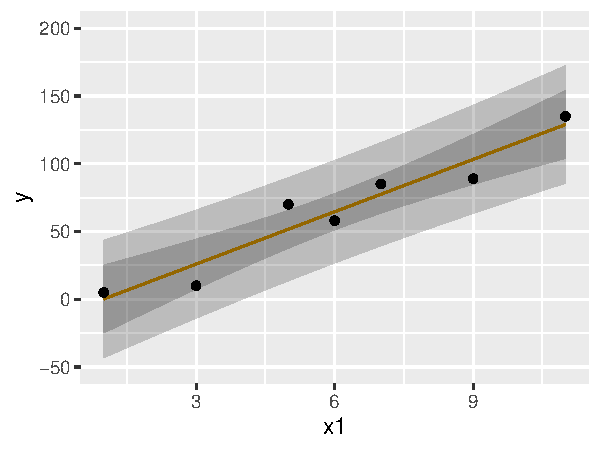
\includegraphics[width=\maxwidth]{reg-both-type-cls-1} }

\caption[Two types of confidence bands]{Pointwise 0.95 confidence intervals for $\hat{y}$ (wider bands) and $\hat{E}(y|x)$ (narrower bands).}\label{fig:reg-both-type-cls}
\end{figure}
\end{Schunk}
\ei
\clearpage

\subsection{Assessing Goodness of Fit}
\ros{11.6} \sound{reg-6} \disc{reg-simple-gof}
Assumptions:
\be
\item   Linearity
\item   $\sigma^2$ is constant, independent of $x$
\item   Observations ($e$'s) are independent of each other
\item   For proper statistical inference (CI, $P$-values), $y$ ($e$)
        is normal conditional on $x$
\ee
Verifying some of the assumptions:
\bi
\item   In a scattergram the spread of $y$ about the fitted line
        should be constant as $x$ increases, and $y$ vs.\ $x$ should
        appear linear
\item   Easier to see this with a plot of $\hat{d} = y - \hat{y}$ vs.\
  $\hat{y}$
\item   In this plot there are no
        systematic patterns (no trend in central tendency, no change
        in spread of points with $x$)
\item Trend in central tendency indicates failure of linearity
\item   \texttt{qqnorm} plot of $d$
\ei
\begin{Schunk}
\begin{Sinput}
# Fit a model where x and y should have been log transformed
n <- 50
set.seed(2)
res <- rnorm(n, sd=.25)
x <- runif(n)
y <- exp(log(x) + res)
f <- ols(y ~ x)
plot(fitted(f), resid(f))    # Fig. (*\ref{fig:reg-exresid}*)
# Fit a linear model that should have been quadratic
x <- runif(n, -1, 1)
y <- x ^ 2 + res
f <- ols(y ~ x)
plot(fitted(f), resid(f))
# Fit a correctly assumed linear model
y <- x + res
f <- ols(y ~ x)
plot(fitted(f), resid(f))
# Q-Q plot to check normality of residuals
qqnorm(resid(f)); qqline(resid(f))
\end{Sinput}
\begin{figure}[htbp]

\centerline{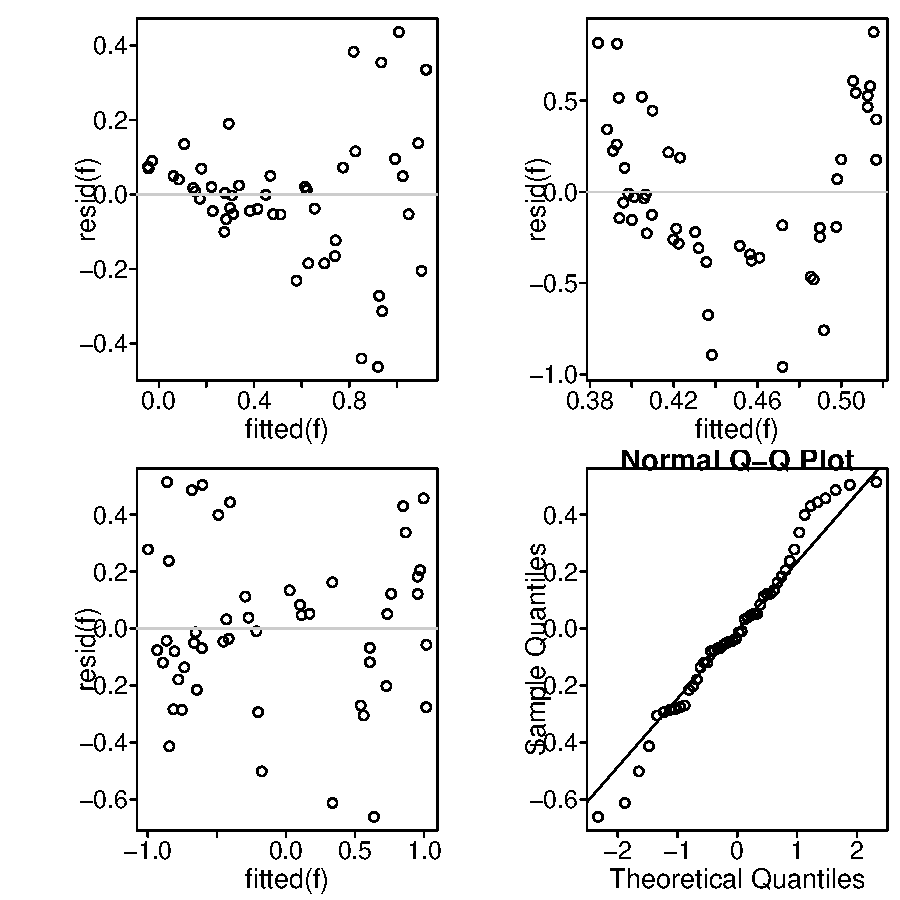
\includegraphics[width=\maxwidth]{reg-exresid-1} }

\caption[Four examples of residual plots]{Using residuals to check some of the assumptions of the simple linear regression model.  Top left panel depicts non-constant $\sigma^2$, which might call for transforming $y$.  Top right panel shows constant variance but the presence of a systemic trend which indicates failure of the linearity assumption.  Bottom left panel shows the ideal situation of white noise (no trend, constant variance).  Bottom right panel shows a $q-q$ plot that demonstrates approximate normality of residuals, for a sample of size $n=50$.  Horizontal reference lines are at zero, which is by definition the mean of all residuals.}\label{fig:reg-exresid}
\end{figure}
\end{Schunk}
\clearpage

\subsection{Summary: Useful Equations for Linear Regression}
Simple linear regression: one predictor ($p=1$): \\
Model:	$E(y|x) = \alpha + \beta x$ \\ $E(y) = $expectation or long--term
	average of $y$ ~~~ $| = $ conditional on \\
Alternate statement of model:	$y = \alpha + \beta x + e,\quad e$
normal with mean zero for all $x$, $\quad var(e) = \sigma^{2} = var(y
| x)$

Assumptions:
\be
\item	Linearity
\item	$\sigma^2$ is constant, independent of $x$
\item	Observations ($e$'s) are independent of each other
\item	For proper statistical inference (CI, $P$--values), $y$ ($e$)
		is normal conditional on $x$
\ee
Verifying some of the assumptions:
\be
\item	In a scattergram the spread of $y$ about the fitted line
		should be constant as $x$ increases
\item	In a residual plot ($d = y - \hat{y}$ vs.\ $x$) there are no
		systematic patterns (no trend in central tendency, no change
		in spread of points with $x$)
\ee

Sample of size $n: (x_{1}, y_{1}), (x_{2}, y_{2}), \ldots, (x_{n},y_{n})$

\ipacue\beqa
L_{xx} = \sum(x_{i}-\bar{x})^2 & L_{xy} = \sum(x_{i}-\bar{x})(y_{i}-\bar{y}) \\
\hat{\beta} = b = \frac{L_{xy}}{L_{xx}}	&	\hat{\alpha} = a = \bar{y}- b \bar{x} \\
\hat{y} = a + bx = \hat{E}(y | x) & \textrm{estimate of~} E(y|x) =
\textrm{~estimate of y} \\
SST = \sum(y_{i} - \bar{y})^{2}	& MST = \frac{SST}{n-1} = s_{y}^{2} \\
SSR = \sum(\hat{y}_{i} - \bar{y})^{2}	&	MSR = \frac{SSR}{p} \\
SSE = \sum(y_{i} - \hat{y_{i}})^{2}		&	MSE = \frac{SSE}{n-p-1} =
s_{y\cdot x}^{2} \\
SST = SSR + SSE							& F = \frac{MSR}{MSE} =
\frac{R^{2}/p}{(1 - R^{2})/(n-p-1)} \sim F_{p,n-p-1} \\
R^{2} = \frac{SSR}{SST}					& \frac{SSR}{MSE} \dot{\sim} \chi^{2}_{p} \\
(p=1) ~~ \widehat{s.e.}(b) = \frac{s_{y \cdot x}}{\sqrt{L_{xx}}} &
	t = \frac{b}{\widehat{s.e.}(b)} \sim t_{n-p-1} \\
1-\alpha \textrm{~two--sided CI for~} \beta & b \pm
t_{n-p-1,1-\alpha/2}\widehat{s.e.}(b) \\
(p=1) ~~ \widehat{s.e.}(\hat{y}) = s_{y \cdot x} \sqrt{1 + \frac{1}{n} +
\frac{(x-\bar{x})^{2}}{L_{xx}}} & \\
1-\alpha \textrm{~two--sided CI for~} y & \hat{y} \pm
t_{n-p-1,1-\alpha/2}\widehat{s.e.}(\hat{y}) \\
(p=1) ~~ \widehat{s.e.}(\hat{E}(y|x)) = s_{y \cdot x} \sqrt{\frac{1}{n} +
\frac{(x-\bar{x})^{2}}{L_{xx}}} \\
1-\alpha \textrm{~two--sided CI for~} E(y|x) & \hat{y} \pm
t_{n-p-1,1-\alpha/2}\widehat{s.e.}(\hat{E}(y|x)) \\
\eeqa

Multiple linear regression: $p$ predictors, $p > 1$: \\
Model: $E(y|x) = \alpha + \beta_{1} x_{1} + \beta_{2} x_{2} + \ldots +
\beta_{p} x_{p} + e$ \\
Interpretation of $\beta_{j}$: effect on $y$ of increasing $x_{j}$ by
one unit, holding all other $x$'s constant \\

Assumptions: same as for $p=1$ plus no interaction between the $x$'s
($x$'s act additively; effect of $x_{j}$ does not depend on the other $x$'s).

Verifying some of the assumptions:
\be
\item	When $p=2$, $x_{1}$ is continuous, and $x_{2}$ is binary, the
		pattern of $y$ vs.\ $x_{1}$, with points identified by
		$x_{2}$, is two straight, parallel lines
\item	In a residual plot ($d = y - \hat{y}$ vs.\ $\hat{y}$) there are no
		systematic patterns (no trend in central tendency, no change
		in spread of points with $\hat{y}$).  The same is true if one
		plots $d$ vs.\ any of the $x$'s.
\item	Partial residual plots reveal the partial (adjusted)
relationship between a chosen $x_{j}$ and $y$, controlling for all
other $x_{i}, i \neq j$, without assuming linearity for $x_{j}$.  In
these plots, the following quantities appear on the axes:
	\begin{description}
	\item[$y$ axis:] residuals from predicting $y$ from all predictors
		except $x_j$
	\item[$x$ axis:] residuals from predicting $x_j$ from all
		predictors except $x_{j}$ ($y$ is ignored)
	\end{description}
\ee

When $p>1$, least squares estimates are obtained using more complex
formulas.  But just as in the case with $p=1$, all of the coefficient
estimates are weighted combinations of the $y$'s, $\sum w_{i}y_{i}$
[when $p=1$, the $w_i$ for estimating $\beta$ are
$\frac{x_{i}-\bar{x}}{\sum(x_{i}-\bar{x})^{2}}$].

Hypothesis tests with $p>1$:
\bi
\item	Overall $F$ test tests $H_{0}: \beta_{1} = \beta_{2} = \ldots
		\beta_{p} = 0$ vs.\ the althernative hypothesis that at least one of
		the $\beta$'s $\neq 0$.
\item	To test whether an individual $\beta_{j}=0$ the simplest
		approach is to compute the $t$ statistic, with $n-p-1$ d.f.
\item	Subsets of the $\beta$'s can be tested against zero if one
		knows the standard errors of all of the estimated coefficients
		and the correlations of each pair of estimates.  The formulas
		are daunting.
\item	To test whether a subset of the $\beta$'s are all zero, a good
		approach is to compare the model containing all of the
		predictors associated with the $\beta$'s of interest with a
		sub--model containing only the predictors not being tested
		(i.e., the predictors being adjusted for).  This tests whether
		the predictors of interest add response information to the
		predictors being adjusted for.  If the goal is to
		test $H_{0}:\beta_{1}=\beta_{2}=\ldots=\beta_{q}=0$ regardless
		of the values of $\beta_{q+1},\ldots,\beta_{p}$ (i.e.,
		adjusting for $x_{q+1},\ldots,x_{p}$), fit the full model with
		$p$ predictors, computing $SSE_{full}$ or $R^{2}_{full}$.  Then
		fit the sub--model omitting $x_{1},\ldots,x_{q}$ to obtain
		$SSE_{reduced}$ or $R^{2}_{reduced}$.  Then compute the
		partial $F$ statistic
		\[
		F = \frac{(SSE_{reduced} - SSE_{full})/q}{SSE_{full}/(n-p-1)}
		= \frac{(R^{2}_{full} - R^{2}_{reduced})/q}{(1 -
		R^{2}_{full})/(n-p-1)} \sim F_{q,n-p-1}
		\]
		Note that $SSE_{reduced} - SSE_{full} = SSR_{full} - SSR_{reduced}$.
\ei

Notes about distributions:
\bi
\item	If $t \sim t_{b}, \quad t \dot{\sim} $ normal for large $b$ and $t^{2}
\dot{\sim} \chi^{2}_{1},$ so [$\frac{b}{\widehat{s.e.}(b)}]^{2} \dot{\sim} \chi^{2}_{1}$
\item	If $F \sim F_{a,b}, \quad a \times F \dot{\sim} \chi^{2}_{a}$ for large $b$
\item	If $F \sim F_{1,b}, \quad \sqrt{F} \sim t_{b}$
\item	If $t \sim t_{b}, \quad t^{2} \sim F_{1,b}$
\item	If $z \sim $ normal,$ \quad z^{2} \sim \chi^{2}_{1}$
\item	$y \sim D$ means $y$ is distributed as the distribution $D$
\item	$y \dot{\sim} D$ means that $y$ is approximately distributed
		as $D$ for large $n$
\item	$\hat{\theta}$ means an estimate of $\theta$
\ei

\ignore{
\section{Multivariable Modeling: General Issues}
\subsection{Planning for Modeling}\rms{1.4}
\bi
\item   Response definition, follow-up, longitudinal vs. single time
\item   Variable definitions
\item   Observer variability
\item   Missing data
\item   Preference for continuous variables
\item   Subjects
\item   Sites
\ei

\subsection{Choice of the Model}\rms{1.5}
\bi
\item   In biostatistics and epidemiology we usually choose model
        empirically
\item   Model must use data efficiently
\item   Should model overall structure (e.g., acute vs.\ chronic)
\item   Robust models are better
\item   Should have correct mathematical structure (e.g., constraints
        on probabilities)
\ei
}   % end ignore

\section{Proper Transformations and Percentiling}\sound{reg-7}
\disc{reg-percentiling}
\bi
\item All parametric and semi-parametric regression models make
  assumptions about the shape of the relationship between predictor
  $X$ and response variable $Y$
\item Many analysts assume linear relationships by default
\item Regression splines (piecewise polynomials) are natural nonlinear
  generalizations
\item In epidemiology and public health many practitioners analyze
  data using percentiling (e.g., of BMI against a random sample of the
  population)
\item This assumes that $X$ affects $Y$ though the population
  distribution of $X$ (e.g., how many persons have BMI similar to a
  subject) instead of through physics, physiology, or anatomy
\item Also allows definitions to change as the population accommodates
\item Example: assume BMI is normal with mean 28 and SD 2\ipacue
\item Figure~\ref{fig:reg-bmi} upper left panel shows this distribution
\item Upper right: percentile of BMI vs.\ raw BMI
\item Lower left: supposed relationship between BMI and disease risk
\item Lower right: resulting relationship between BMI percentile and risk
\ei
All parametric regression models make assumptions about the form of
the relationship between the predictors $X$ and the response variable
$Y$.  The typical default assumption is linearity in $X$ vs.\ some
transformation of $Y$ (e.g., log odds, log hazard or in ordinary
regression the identify function).  Regression splines are one of the
best approaches for allowing for smooth, flexible regression function
shapes.  Splines are described in detail in the \emph{Regression
  Modeling Strategies} book and course notes.

Some researchers and government agencies get the idea that continuous
variables should be modeled through percentiling.  This is a rather
bizarre way to attempt to account for shifts in the distribution of
the variable by age, race, sex, or geographic location.  Percentiling
fails to recognize that the way that measurements affect subjects'
responses is through physics, physiology, anatomy, and other means.
Percentiling in effect states that how a variable affects the outcome
for a subject depends on how many other subjects there are like her.
When also percentiling variables (such as BMI) over time, the
measurement even changes its meaning over time.  For example, updating
percentiles of BMI each year will keep the fraction of obese members
in the population constant even when obesity is truly on the rise.

Putting percentiles into a regression model assumes that the shape of
the $X-Y$ relationship is a very strange.  As an example, suppose that
BMI has a normal distribution with mean 28 and standard deviation 2.
The density function for BMI is shown in the upper left panel of
Figure~\ref{fig:reg-bmi}, and the function giving the percentile of
BMI as a function of absolute BMI is in the upper right panel.
\begin{Schunk}
\begin{Sinput}
x <- seq(10, 55, length=200)
d <- dnorm(x, mean=28, sd=2)
plot(x, d, type='l', xlab='BMI', ylab='Density')   # Fig. (*\ref{fig:reg-bmi}*)
pctile <- 100*pnorm(x, mean=28, sd=2)
plot(x, pctile, type='l', xlab='BMI', ylab='BMI Percentile')
risk <- .01 + pmax(x - 25, 0)*.01
plot(x, risk, type='l', xlab='BMI', ylab='Risk')
plot(pctile, risk, type='l', xlab='BMI Percentile', ylab='Risk')
\end{Sinput}
\begin{figure}[htbp]

\centerline{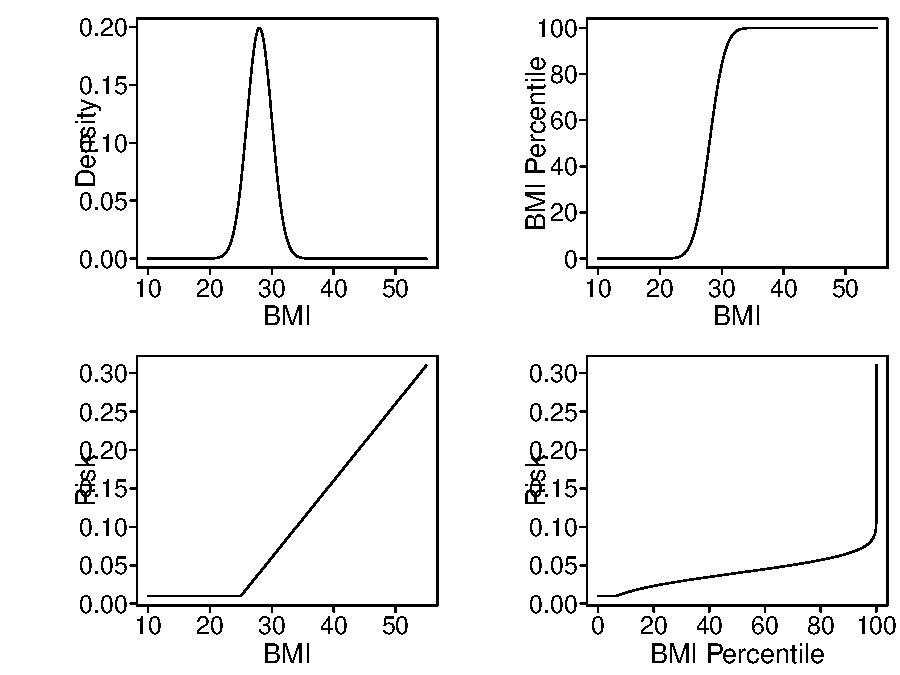
\includegraphics[width=\maxwidth]{reg-bmi-1} }

\caption[Harm of percentiling BMI in a regression model]{Harm of percentiling BMI in a regression model}\label{fig:reg-bmi}
\end{figure}
\end{Schunk}
Suppose that the true relationship between BMI and the risk of a
disease is given in the lower left panel.  Then the relationship
between BMI percentile and risk must be that shown in the lower right
panel.  To properly model that shape one must ``undo'' the percentile
function then fit the result with a linear spline.  Percentiling
creates unrealistic fits and results in more effort being spent if one
is to properly model the predictor.

\bi
\item Worse still is to group $X$ into quintiles and use a linear
  model in the quintile numbers
  \bi
  \item assumes are bizarre shape of relationship between $X$ and $Y$,
    even if not noticing the discontinuities
  \ei
\item Figure~\ref{fig:reg-bmiq} depicts quantile numbers vs.\ mean BMI
  within each quintile.  Outer quintiles:
  \bi
  \item have extremely skewed BMI distributions
  \item are too heterogeneous to yield adequate BMI adjustment
    (residual confounding)
  \ei
\item Easy to see that the transformation of BMI that yields quintile
  numbers is discontinuous with variable step widths
\ei

In epidemiology a common practice is even more problematic.  One often
\ipacue
sees smoothly-acting continuous variables such as BMI broken into
discontinuous quintile \emph{groups}, the groups numbered from 1~to~5,
and a linear regression of correlation fitted to the 1--5 variable
(``test for trend'').
This is not only hugely wasteful of information and power, but results
in significant heterogeneity (especially in the outer quintiles) and
assumes a discontinuous effect on outcome that has an exceedingly
unusual shape when interpreted on the original BMI scale.

Taking the BMI distribution in Figure~\ref{fig:reg-bmi} consider what
this implies.  We draw a random sample of size 500 from
the BMI distribution.  Figure~\ref{fig:reg-bmiq} shows the
discontinuous relationship between BMI and quintile interval.  The
location of the mean BMI within BMI quintile is a circle on each
horizontal line.  One can see the asymmetry of the BMI distribution
in the outer quintiles, and that the meaning of inner quantiles is
fundamentally different than the meaning of the outer ones because of
the narrow range of BMI for inner quantile groups.
\begin{Schunk}
\begin{Sinput}
set.seed(1)
bmi  <- rnorm(500, mean=28, sd=2)
require(Hmisc)
bmiq <- cut2(bmi, g=5)
table(bmiq)
\end{Sinput}
\begin{Soutput}
bmiq
[22.0,26.5) [26.5,27.5) [27.5,28.6) [28.6,29.8) [29.8,35.6] 
        100         100         100         100         100 
\end{Soutput}
\begin{Sinput}
cuts <- cut2(bmi, g=5, onlycuts=TRUE)
cuts
\end{Sinput}
\begin{Soutput}
[1] 21.98390 26.51345 27.48995 28.55872 29.76222 35.62055
\end{Soutput}
\begin{Sinput}
bmim <- cut2(bmi, g=5, levels.mean=TRUE)
means <- as.numeric(levels(bmim))
plot(c(21, 36), c(1, 5), type='n', xlab='BMI', ylab='Quintile #')   # Fig. (*\ref{fig:reg-bmiq}*)
for(i in 1 : 5) {
  lines(cuts[c(i, i+1)], c(i, i))
  points(means[i], i)
}
\end{Sinput}
\begin{figure}[htbp]

\centerline{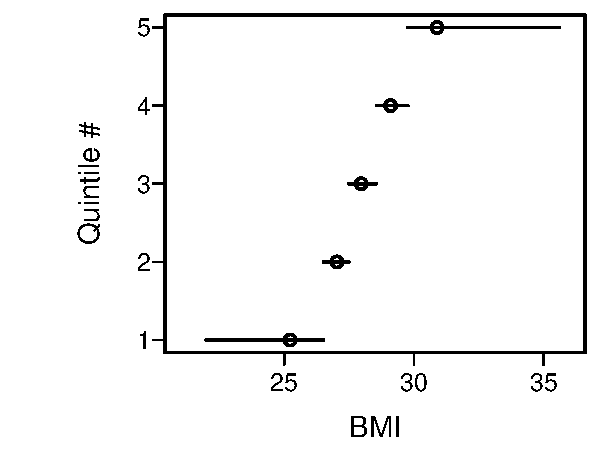
\includegraphics[width=\maxwidth]{reg-bmiq-1} }

\caption[What are quintile numbers modeling?]{What are quintile numbers modeling?}\label{fig:reg-bmiq}
\end{figure}
\end{Schunk}

\clearpage
\section{Multiple Linear Regression}\ems{11}\ros{11.9}\abd{18}
\rms{2.1-2.3} \disc{reg-mult}
\subsection{The Model and How Parameters are Estimated}\sound{reg-8}
\bi
\item $p$ independent variables $x_{1}, x_{2}, \ldots, x_{p}$
\item Examples: multiple risk factors, treatment
  plus patient descriptors when adjusting for non-randomized treatment
  selection in an observational study; a set of controlled or
  uncontrolled factors in an experimental study; indicators of
  multiple experimental manipulations performed simultaneously
\item Each variable has its own effect (slope) representing
  \emph{partial effects}: effect of increasing a variable by one unit,
  holding all others constant
\item Initially assume that the different variables act in an additive
  fashion
\item Assume the variables act linearly against $y$
\item Model: $y = \alpha + \beta_{1}x_{1} + \beta_{2}x_{2} + \ldots +
  \beta_{p}x_{p} + e$ \ipacue
\item Or: $E(y|x) = \alpha + \beta_{1}x_{1} + \beta_{2}x_{2} + \ldots +
  \beta_{p}x_{p}$
\item For two $x$-variables: $y = \alpha + \beta_{1}x_{1} + \beta_{2}x_{2}$
\item Estimated equation: $\hat{y} = a + b_{1}x_{1} + b_{2}x_{2}$
\item Least squares criterion for fitting the model (estimating the
  parameters): \\
  $SSE = \sum_{i=1}^{n} [y - (a + b_{1}x_{1} + b_{2}x_{2})]^2$
\item Solve for $a, b_{1}, b_{2}$ to minimize $SSE$
\item When $p>1$, least squares estimates require complex
formulas; still all of the coefficient estimates are weighted
combinations of the $y$'s, $\sum w_{i}y_{i}$\footnote{When $p=1$, the
  $w_i$ for estimating $\beta$ are
  $\frac{x_{i}-\bar{x}}{\sum(x_{i}-\bar{x})^{2}}$}.
\ei

\subsection{Interpretation of Parameters}\sound{reg-9}
\bi
\item Regression coefficients are ($b$) are commonly called
  \emph{partial regression coefficients}: effects of each variable
  holding all other variables in the model constant
\item Examples of partial effects:
 \bi
 \item model containing $x_1$=age (years) and $x_2$=sex
  (0=male 1=female) \\
  Coefficient of age ($\beta_1$) is the change in the mean of
  $y$ for males when age increases by 1 year.  It is also the change
  in $y$ per unit increase in age for females.  $\beta_2$ is the
  female minus male mean difference in $y$ for two subjects of the
  same age.
  \item $E(y|x_{1},x_{2})=\alpha+\beta_{1}x_{1}$ for males,
    $\alpha+\beta_{1}x_{1}+\beta_{2} =
    (\alpha+\beta_{2})+\beta_{1}x_{1}$ for females [the sex effect is
    a shift effect or change in $y$-intercept]
  \item model with age and systolic blood pressure measured when the
   study begins \\
   Coefficient of blood pressure is the change in mean $y$ when blood
   pressure increases by 1mmHg for subjects of the same age
  \ei
\item What is meant by changing a variable? \ipacue
 \bi
 \item We usually really mean a comparison of two subjects with
   different blood pressures
 \item Or we can envision what would be the expected response had
   \emph{this} subject's blood pressure been 1mmHg greater at the
   outset\footnote{This setup is the basis for randomized controlled
     trials and randomized animal experiments.  Drug effects may be
     estimated with between-patient group differences under a
     statistical model.}
 \item We are not speaking of longitudinal changes in a single
   person's blood pressure
 \item We can use subtraction to get the adjusted (partial) effect of
   a variable, e.g., $E(y|x_{1}=a+1,x_{2}=s)-E(y|x_{1}=a, x_{2}=s) =\\
   \alpha + \beta_{1}(a+1) + \beta_{2}s -
   (\alpha + \beta_{1}a + \beta_{2}s) = \beta_{1}$
 \ei
\item Example: $\hat{y} = 37 + .01\times\textrm{weight} +
  0.5\times\textrm{cigarettes smoked per day}$ \ipacue
 \bi
 \item .01 is the estimate of average increase $y$ across subjects
   when weight is
   increased by 1lb.\ if cigarette smoking is unchanged
 \item 0.5 is the estimate of the average increase in $y$ across
   subjects per additional cigarette smoked per day if weight does not
   change
 \item 37 is the estimated mean of $y$ for a subject of zero weight
   who does not smoke
 \ei
\item Comparing regression coefficients:
 \bi
 \item Can't compare directly because of different units of
   measurement.  Coefficients in units of $\frac{y}{x}$.
 \item Standardizing by standard deviations: not recommended.  Standard
   deviations are not magic summaries of scale and they give the wrong
   answer when an $x$ is categorical (e.g., sex).
 \ei
\ei

\subsection{Example: Estimation of Body Surface Area}\sound{reg-9a}
DuBois \& DuBois developed an equation in log height and log
weight in 1916 that is still used\footnote{DuBois D, DuBois EF: A
  formula to estimate the approximate surface area if height and
  weight be known.  \emph{Arch Int Medicine} \textbf{17}(6):863-71,
  1916.}.  We use the main data they used\footnote{A Stata data file
  \co{dubois.dta} is available \href{http://biostat.mc.vanderbilt.edu/wiki/pub/Main/DataSets/dubois.dta}{here}.}.

\begin{Schunk}
\begin{Sinput}
require(rms)
d <- read.csv(textConnection(
'weight,height,bsa
24.2,110.3,8473
64.0,164.3,16720
64.1,178.0,18375
74.1,179.2,19000
93.0,149.7,18592
45.2,171.8,14901
32.7,141.5,11869
6.27,73.2,3699
57.6,164.8,16451
63.0,184.2,17981'))
d <- upData(d, labels=c(weight='Weight', height='Height',
                        bsa='Body Surface Area'),
            units=c(weight='kg', height='cm', bsa='cm^2'), print=FALSE)
d
\end{Sinput}
\begin{Soutput}
   weight height   bsa
1   24.20  110.3  8473
2   64.00  164.3 16720
3   64.10  178.0 18375
4   74.10  179.2 19000
5   93.00  149.7 18592
6   45.20  171.8 14901
7   32.70  141.5 11869
8    6.27   73.2  3699
9   57.60  164.8 16451
10  63.00  184.2 17981
\end{Soutput}
\begin{Sinput}
# Create Stata file
getRs('r2stata.r', put='source')
dubois <- d
r2stata(dubois)
\end{Sinput}
\begin{Sinput}
# Exclude subject measured using adhesive plaster method
d <- d[-7, ]
\end{Sinput}
\end{Schunk}
Fit a multiple regression model in the logs of all 3 variables\ipacue
\begin{Sinput}
dd <- datadist(d); options(datadist='dd')
f <- ols(log10(bsa) ~ log10(weight) + log10(height), data=d)
f
\end{Sinput}

 \centerline{\textbf{Linear Regression Model}}
 
 \begin{verbatim}
 ols(formula = log10(bsa) ~ log10(weight) + log10(height), data = d)
 \end{verbatim}
 
 {\fontfamily{phv}\selectfont \begin{center}\begin{tabular}{|c|c|c|}\hline
&Model Likelihood&Discrimination\\
&Ratio Test&Indexes\\\hline
Obs~\hfill 9&LR $\chi^{2}$~\hfill 66.23&$R^{2}$~\hfill 0.999\\
$\sigma$~\hfill 0.0069&d.f.~\hfill 2&$R^{2}_{\textrm{adj}}$~\hfill 0.999\\
d.f.~\hfill 6&Pr$(>\chi^{2})$~\hfill 0.0000&$g$~\hfill 0.226\\
\hline
\end{tabular}
\end{center}}
 \begin{center}
 Residuals
 

 \begin{tabular}{ccccc}
Min&1Q&Median&3Q&Max\\
$-0.005031$&$-0.004851$&$-0.001908$&$0.002541$&$0.01198$\\
\end{tabular}
 \end{center}
 
 %latex.default(U, file = "", first.hline.double = FALSE, table = FALSE,     longtable = TRUE, lines.page = lines.page, col.just = rep("r",         ncol(U)), rowlabel = "", already.math.col.names = TRUE,     append = TRUE)%
 \setlongtables\begin{longtable}{lrrrr}\hline
 \multicolumn{1}{l}{}&\multicolumn{1}{c}{$\hat{\beta}$}&\multicolumn{1}{c}{S.E.}&\multicolumn{1}{c}{$t$}&\multicolumn{1}{c}{Pr$(>|t|)$}\tabularnewline
 \hline
 \endhead
 \hline
 \endfoot
 Intercept&~1.9607~&~0.0808~&24.26&\textless 0.0001\tabularnewline
 weight&~0.4198~&~0.0184~&22.77&\textless 0.0001\tabularnewline
 height&~0.6812~&~0.0499~&13.64&\textless 0.0001\tabularnewline
 \hline
 \end{longtable}
 \addtocounter{table}{-1}

DuBois \& DuBois derived the equation log(bsa) = 1.8564 + 0.426
log(weight) + 0.725 log(height)

Plot predicted vs.\ observed
\begin{Schunk}
\begin{Sinput}
plot(fitted(f), log10(d$bsa), xlab=expression(hat(Y)),
     ylab=expression(log[10](BSA))); abline(a=0, b=1, col=gray(.85))
\end{Sinput}


\centerline{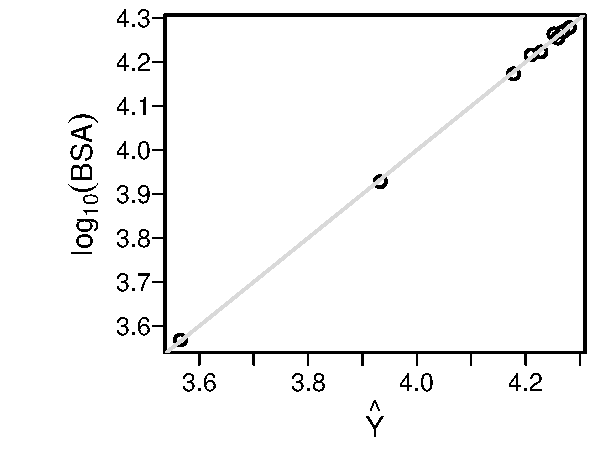
\includegraphics[width=\maxwidth]{reg-dreg2-1} }

\end{Schunk}

Get 3 types of plots to show fitted model\ipacue
\begin{Schunk}
\begin{Sinput}
p <- Predict(f, weight=seq(5, 100, length=50),
             height=seq(70, 190, length=50), fun=function(z) 10 ^ z)
p1 <- bplot(p)
p2 <- bplot(p, lfun=contourplot, cuts=20)
arrGrob(p1, p2, ncol=2)
\end{Sinput}


\centerline{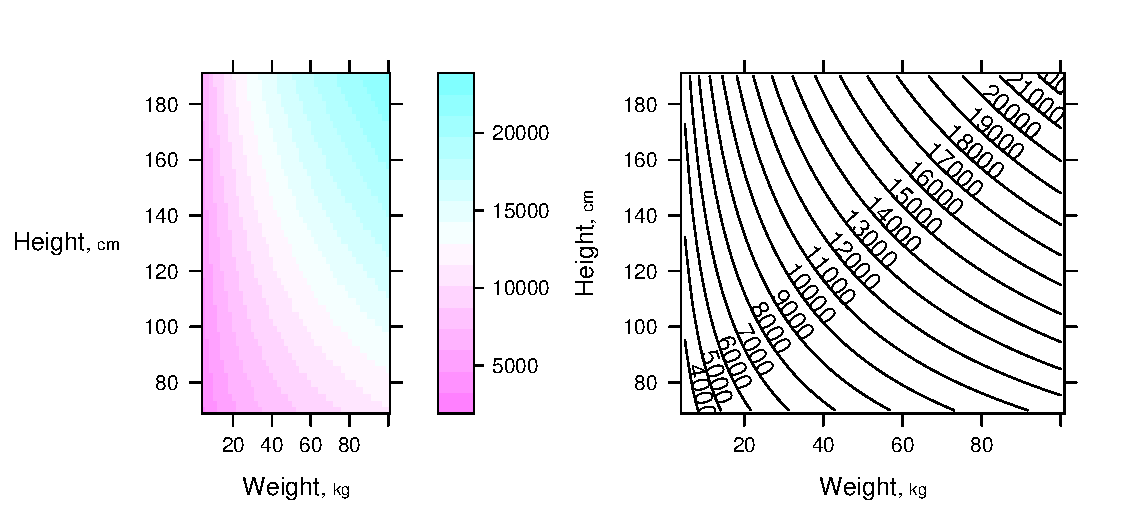
\includegraphics[width=\maxwidth]{reg-dreg3-1} }

\end{Schunk}
\begin{Schunk}
\begin{Sinput}
bplot(p, lfun=wireframe, zlab='BSA')
\end{Sinput}


\centerline{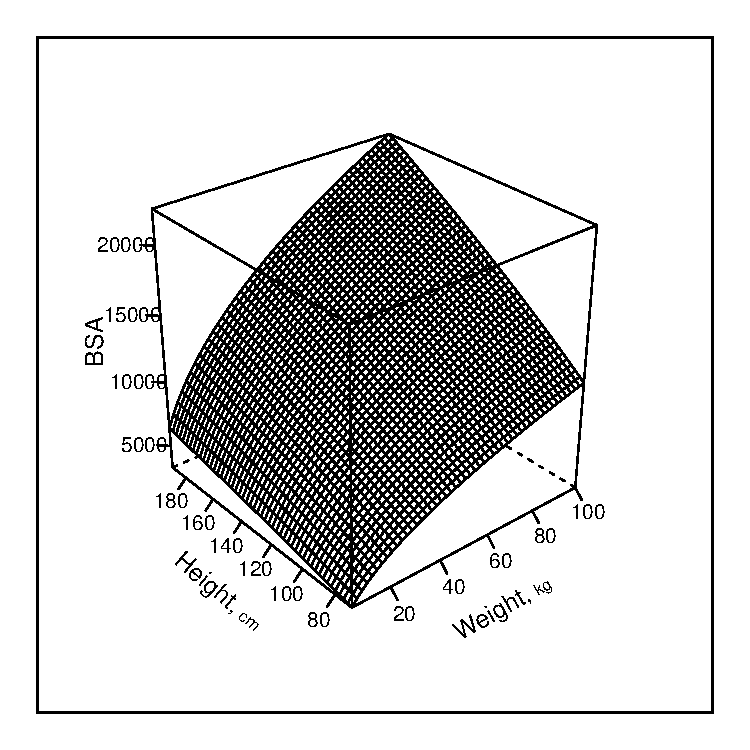
\includegraphics[width=\maxwidth]{reg-dreg4-1} }

\end{Schunk}
Note: this plot would be a plane if all 3 variables were plotted on
the scale fitted in the regression ($\log_{10}$).

\subsection{What are Degrees of Freedom}\sound{reg-10}
\bd
\item[For a model]: the total number of parameters not counting
  intercept(s)
\item[For a hypothesis test]: the number of parameters that are
  hypothesized to equal specified constants.  The constants specified
  are usually zeros (for \emph{null} hypotheses) but this is not
  always the case.  Some tests involve combinations of multiple
  parameters but test this combination against a single constant; the
  d.f.\ in this case is still one.  Example: $H_{0}:
  \beta_{3}=\beta_{4}$ is the same as $H_{0}:\beta_{3}-\beta_{4}=0$
  and is a 1 d.f.\ test because it tests one parameter
  ($\beta_{3}-\beta_{4}$) against a constant ($0$).
\ed

These are \textbf{numerator d.f.} in the sense of the $F$-test in
multiple linear regression.  The $F$-test also entails a second kind
of d.f., the \textbf{denominator} or \textbf{error} d.f., $n-p-1$,
where $p$ is the number of parameters aside from the intercept.  The
error d.f.\ is the denominator of the estimator for $\sigma^2$ that is
used to unbias the estimator, penalizing for having estimated $p+1$
parameters by minimizing the sum of squared errors used to estimate
$\sigma^2$ itself.  You can think of the error d.f.\ as the sample
size penalized for the number of parameters estimated, or as a measure
of the information base used to fit the model.

Other ways to express the d.f.\ for a hypothesis are:
\bi
\item The number of opportunities you give associations to be present (relationships with $Y$ to be non-flat)
\item The number of restrictions you place on parameters to make the null hypothesis of no association (flat relationships) hold
\ei

\subsection{Hypothesis Testing} \ems{11.2}\ros{11.9.2}
\disc{reg-mult-h0}
\subsubsection{Testing Total Association (Global Null Hypotheses)}
\bi
\item ANOVA table is same as before for general $p$
\item $F_{p, n-p-1}$ tests $H_{0}:
  \beta_{1}=\beta_{2}=\ldots=\beta_{p}=0$
\item This is a test of \emph{total association}, i.e., a test of
  whether \emph{any} of the predictors is associated with $y$
\item To assess total association we accumulate partial effects of all
  variables in the model \emph{even though} we are testing if
  \emph{any} of the partial effects is nonzero
\item $H_{a}:$ at least one of the $\beta$'s is non-zero.
  \textbf{Note}: This does not mean that all of the $x$ variables are
  associated with $y$.
\item Weight and smoking example: $H_{0}$ tests the null hypothesis
  that neither weight nor smoking is associated with $y$.  $H_{a}$ is
  that at least one of the two variables is associated with $y$.  The
  other may or may not have a non-zero $\beta$.
\item Test of total association does not test whether cigarette
  smoking is related to $y$ holding weight constant.
\item $SSR$ can be called the model $SS$
\ei

\subsubsection{Testing Partial Effects}\sound{reg-11}\disc{reg-mult-h0-partial}
\bi
\item $H_{0}: \beta_{1}=0$ is a test for the effect of $x_{1}$ on $y$
  holding $x_{2}$ and any other $x$'s constant
\item Note that $\beta_{2}$ is \emph{not} part of the null or
  alternative hypothesis; we assume that we have adjusted for
  \emph{whatever} effect $x_{2}$ has, \emph{if any}
\item One way to test $\beta_{1}$ is to use a $t$-test:
  $t_{n-p-1} = \frac{b_{1}}{\widehat{s.e.}(b_{1})}$
\item In multiple regression it is difficult to compute standard
  errors so we use a computer
\item These standard errors, like the one-variable case, decrease when
 \bi
 \item $n \uparrow$
 \item variance of the variable being tested $\uparrow$
 \item $\sigma^{2}$ (residual $y$-variance) $\downarrow$
 \ei
\item Another way to get partial tests: the $F$ test \ipacue
 \bi
 \item Gives identical 2-tailed $P$-value to $t$ test when one $x$
   being tested \\ $t^{2} \equiv$ partial $F$
 \item Allows testing for $> 1$ variable
 \item Example: is either systolic or diastolic blood pressure (or
   both) associated with the time until a stroke, holding weight constant
 \ei
\item To get a partial $F$ define partial $SS$
\item Partial $SS$ is the change in $SS$ when the variables
  \textbf{being tested} are dropped from the model and the model is
  re-fitted
\item A general principle in regression models: a set of variables can
  \ipacue
  be tested for their combined partial effects by removing that set of
  variables from the model and measuring the harm ($\uparrow SSE$)
  done to the model
\item Let $full$ refer to computed values from the full model
  including all variables; $reduced$ denotes a reduced model
  containing only the adjustment variables and not the variables being
  tested
\item Dropping variables $\uparrow SSE, \downarrow SSR$ unless the
  dropped variables had exactly zero slope estimates in the full model
  (which never happens)
\item $SSE_{reduced} - SSE_{full} = SSR_{full} - SSR_{reduced}$ \\
  Numerator of $F$ test can use either $SSE$ or $SSR$
\item Form of partial $F$-test: change in $SS$ when dropping the
  variables of interest divided by change in d.f., then divided by
  $MSE$; \\
  $MSE$ is chosen as that which best estimates $\sigma^2$, namely the
  $MSE$ from the full model
\item Full model has $p$ slopes; suppose we want to test $q$ of the
  slopes
\ipacue\beqa
F_{q, n-p-1} &=& \frac{(SSE_{reduced} - SSE_{full})/q}{MSE} \\
            &=& \frac{(SSR_{full} - SSR_{reduced})/q}{MSE}
\eeqa
\ei

\subsection{Assessing Goodness of Fit}
\ems{12} \ros{11.9.3} \sound{reg-12} \disc{reg-mult-gof}
Assumptions:
\bi
\item   Linearity of each predictor against $y$ holding others constant
\item   $\sigma^2$ is constant, independent of $x$
\item   Observations ($e$'s) are independent of each other
\item   For proper statistical inference (CI, $P$-values), $y$ ($e$)
        is normal conditional on $x$
\item $x$'s act additively; effect of $x_{j}$ does not depend on the
  other $x$'s (\textbf{But} note that the $x$'s may be correlated with
  each other without affecting what we are doing.)
\ei

Verifying some of the assumptions:
\be
\item   When $p=2$, $x_{1}$ is continuous, and $x_{2}$ is binary, the
        pattern of $y$ vs.\ $x_{1}$, with points identified by
        $x_{2}$, is two straight, parallel lines.  $\beta_{2}$ is the
        slope of $y$ vs.\ $x_{2}$ holding $x_{1}$ constant, which is
        just the difference in means for $x_{2}=1$ vs.\ $x_{2}=0$ as
        $\Delta x_{2}=1$ in this simple case.
\begin{Schunk}
\begin{Sinput}
# Generate 25 observations for each group, with true beta1=.05, true beta2=3
d <- expand.grid(x1=1:25, x2=c(0, 1))
set.seed(3)
d$y <- with(d, .2*x1 + 3*x2 + rnorm(50, sd=.5))
with(d, plot(x1, y, xlab=expression(x[1]), ylab=expression(y)))
abline(a=0, b=.2)    # Fig. (*\ref{fig:reg-mult-reg-assume-twovar}*)
abline(a=3, b=.2)
text(13, 1.3, expression(y==alpha + beta[1]*x[1]),           srt=24, cex=1.3)
text(13, 7.1, expression(y==alpha + beta[1]*x[1] + beta[2]), srt=24, cex=1.3)
\end{Sinput}
\begin{figure}[htbp]

\centerline{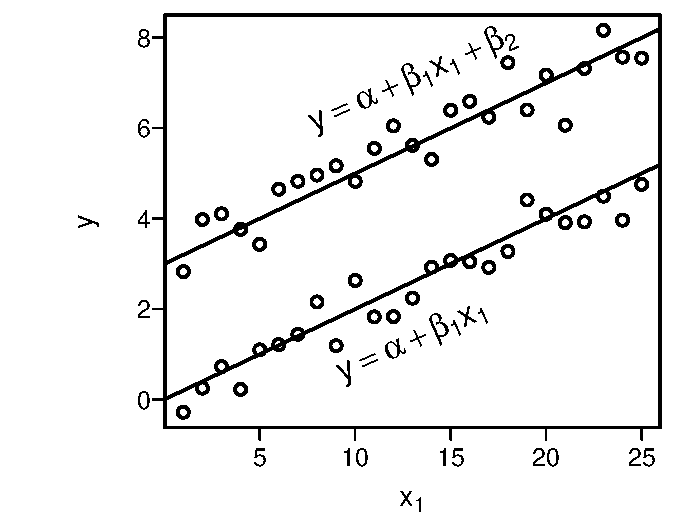
\includegraphics[width=\maxwidth]{reg-mult-reg-assume-twovar-1} }

\caption[Assumptions for two predictors]{Data satisfying all the assumptions of simple multiple linear regression in two predictors.  Note equal spread of points around the population regression lines for the $x_{2}=1$ and $x_{2}=0$ groups (upper and lower lines, respectively) and the equal spread across $x_1$.  The $x_{2}=1$ group has a new intercept, $\alpha+\beta_2$, as the $x_2$ effect is $\beta_2$.  On the $y$ axis you can clearly see the difference between the two true population regression lines is $\beta_{2} = 3$.}\label{fig:reg-mult-reg-assume-twovar}
\end{figure}
\end{Schunk}
\item   In a residual plot ($d = y - \hat{y}$ vs.\ $\hat{y}$) there are no
        systematic patterns (no trend in central tendency, no change
        in spread of points with $\hat{y}$).  The same is true if one
        plots $d$ vs.\ any of the $x$'s (these are more stringent
        assessments).  If $x_{2}$ is binary box plots of $d$
        stratified by $x_{2}$ are effective.
\item   Partial residual plots reveal the partial (adjusted)
relationship between a chosen $x_{j}$ and $y$, controlling for all
other $x_{i}, i \neq j$, without assuming linearity for $x_{j}$.  In
these plots, the following quantities appear on the axes:
    \begin{description}
    \item[$y$ axis:] residuals from predicting $y$ from all predictors
        except $x_j$
    \item[$x$ axis:] residuals from predicting $x_j$ from all
        predictors except $x_{j}$ ($y$ is ignored)
    \end{description}
Partial residual plots ask how does what we can't predict about $y$
without knowing $x_j$ depend on what we can't predict about $x_j$ from
the other $x$'s.
\ee
\clearpage

\section{Multiple Regression with a Binary Predictor}\ros{11.10}\disc{reg-xbinary}
\subsection{Indicator Variable for Two-Level Categorical Predictors}%
\sound{reg-13}
\bi
\item Categories of predictor: $A, B$ (for example)
\item First category = reference cell, gets a zero
\item Second category gets a 1.0
\item Formal definition of indicator (dummy) variable: $x = [category=B]$ \\
  $[w]=1$ if $w$ is true, 0 otherwise
\item $\alpha + \beta x = \alpha + \beta [category=B]$ = \\
  $\alpha$ for category $A$ subjects \\
  $\alpha + \beta$ for category $B$ subjects \\
  $\beta$ = mean difference ($B - A$)
\ei

\subsection{Two-Sample $t$-test vs.\ Simple Linear Regression}
\bi
\item They are equivalent in every sense:
  \bi
  \item $P$-value
  \item Estimates and C.L.s after rephrasing the model
  \item Assumptions (equal variance assumption of two groups in
    $t$-test is the same as constant variance of $y | x$ for every
    $x$)
  \ei
\item $a = \bar{Y}_{A}$ \\
  $b = \bar{Y}_{B} - \bar{Y}_{A}$
\item $\widehat{s.e.}(b) = \widehat{s.e.}(\bar{Y}_{B} - \bar{Y}_{A})$
\ei

\subsection{Analysis of Covariance}\sound{reg-14}\disc{reg-ancova}
\bi
\item Multiple regression can extend the $t$-test
 \bi
 \item More than 2 groups (multiple indicator variables can do
   multiple-group ANOVA)
 \item Allow for categorical or continuous adjustment variables
   (covariates, covariables)
 \ei
\item Example: lead exposure and neuro-psychological function (Rosner)
\item Model: $MAXFWT = \alpha + \beta_{1} age + \beta_{2} sex + e$
\item Rosner coded $sex=1, 2$ for male, female \\
  Does not affect interpretation of $\beta_2$ but makes interpretation
  of $\alpha$ more tricky (mean $MAXFWT$ when $age=0$ and $sex=0$
  which is impossible by this coding.
\item Better coding would have been $sex=0, 1$ for male, female
 \bi
 \item $\alpha$ = mean $MAXFWT$ for a zero year-old male
 \item $\beta_{1}$ = increase in mean $MAXFWT$ per 1-year increase in
   $age$
 \item $\beta_{2} =$ mean $MAXFWT$ for females minus mean $MAXFWT$ for
   males, holding $age$ constant
 \ei
\item Suppose that we define an (arbitrary) \co{exposure} variable to \ipacue
  mean that the lead dose $\geq$ 40mg/100ml in either 1972 \textbf{or} 1973
\item Model: $MAXFWT = \alpha + \beta_{1} exposure + \beta_{2} age +
  \beta_{3} sex + e$ \\
 \Co{exposure} = \Co{TRUE} (1) for exposed, \Co{FALSE} (0) for unexposed
\item $\beta_{1}$ = mean $MAXFWT$ for exposed minus mean for
  unexposed, holding $age$ and $sex$ constant
%\item Pay attention to Rosner's
% \bi
% \item $t$ and $F$ statistics and what they test
% \item Figure 11.28 for checking for trend and equal variability of
%   residuals (don't worry about standardizing residuals)
% \ei
\ei

\section{The Correlation Coefficient Revisited} \ros{11.7}\sound{reg-15}\disc{reg-corr}
Pearson product-moment linear correlation coefficient:
\ipacue\beqa
r &=& \frac{L{xy}}{\sqrt{L_{xx}L_{yy}}} \\
  &=& \frac{s_{xy}}{s_{x}s_{y}} \\
  &=& b \sqrt{\frac{L_{xx}}{L_{yy}}}
\eeqa
\bi
\item $r$ is unitless
\item $r$ estimates the population correlation coefficient $\rho$ (not
  to be confused with Spearman $\rho$ rank correlation coefficient)
\item $-1 \leq r \leq 1$
\item $r = -1$ : perfect negative correlation
\item $r = 1$  : perfect positive correlation
\item $r = 0$  : no correlation (no association)
\item $t-test$ for $r$ is identical to $t$-test for $b$
\item $r^2$ is the proportion of variation in $y$ explained by
  conditioning on $x$
\item $(n-2) \frac{r^{2}}{1-r^{2}} = F_{1,n-2} = \frac{MSR}{MSE}$
\item For multiple regression in general we use $R^2$ to denote the\ipacue
  fraction of variation in $y$ explained jointly by all the $x$'s
  (variation in $y$ explained by the whole model)
\item $R^{2} = \frac{SSR}{SST} = 1 - \frac{SSE}{SST} = 1 $ minus
  fraction of unexplained variation
\item $R^{2}$ is called the \emph{coefficient of determination}
\item $R^2$ is between 0 and 1
 \bi
 \item 0 when $\hat{y}_{i} = \bar{y}$ for all $i$; $SSE=SST$
 \item 1 when $\hat{y}_{i} = y_{i}$ for all $i$; SSE=0
 \ei
\item $R^{2} \equiv r^{2}$ in the one-predictor case
\ei

\section{Using Regression for ANOVA} \ems{9}\ros{12.5.2}\abd{18.1}\disc{reg-anova}
\subsection{Indicator Variables}\sound{reg-16}
\Co{Lead Exposure Group} (Rosner \co{lead} dataset):
\bd
\item[control]: normal in both 1972 and 1973
\item[currently exposed]: elevated serum lead level in 1973, normal in 1972
\item[previously exposed]: elevated lead in 1972, normal in 1973
\ed
\textbf{NOTE}: This is not a very satisfactory way to analyze the two years' worth of lead exposure data, as we do not expect a discontinuous relationship between lead levels and neurological function.  A continuous analysis was done in Chapter~\ref{chap:rmsintro}.
\bi
\item Requires two indicator (dummy) variables (and 2 d.f.) to perfectly describe
  3 categories
\item $x_{1} = [$currently exposed$]$
\item $x_{2} = [$previously exposed$]$
\item Reference cell is control
\item \Co{lead} dataset \Co{group} variable is set up this way already
\item Model:
\ei
\ipacue\beqa
E(y|exposure)  &=& \alpha + \beta_{1}x_{1} +  \beta_{2}x_{2} \\
               &=& \alpha, \textrm{controls} \\
               &=& \alpha + \beta_{1}, \textrm{currently exposed} \\
               &=& \alpha + \beta_{2}, \textrm{previously exposed}
\eeqa
\bd
\item[$\alpha$]: mean \Co{maxfwt} for controls
\item[$\beta_{1}$]: mean \Co{maxfwt} for currently exposed minus mean
  for controls
\item[$\beta_{2}$]: mean \Co{maxfwt} for previously exposed minus mean
  for controls
\item[$\beta_{2} - \beta_{1}$]: mean for previously exposed minus mean
  for currently exposed
\ed
\begin{Sinput}
getHdata(lead)
dd <- datadist(lead); options(datadist='dd')
f <- ols(maxfwt ~ group, data=lead)
f
\end{Sinput}

 \centerline{\textbf{Linear Regression Model}}
 
 \begin{verbatim}
 ols(formula = maxfwt ~ group, data = lead)
 \end{verbatim}
 
 \begin{center}
 Frequencies of Missing Values Due to Each Variable
 
 \smallskip
 
 \begin{verbatim}
 maxfwt  group 
     25      0 
 \end{verbatim}
 
 \end{center}
 {\fontfamily{phv}\selectfont \begin{center}\begin{tabular}{|c|c|c|}\hline
&Model Likelihood&Discrimination\\
&Ratio Test&Indexes\\\hline
Obs~\hfill 99&LR $\chi^{2}$~\hfill 10.33&$R^{2}$~\hfill 0.099\\
$\sigma$~\hfill 12.3127&d.f.~\hfill 2&$R^{2}_{\textrm{adj}}$~\hfill 0.080\\
d.f.~\hfill 96&Pr$(>\chi^{2})$~\hfill 0.0057&$g$~\hfill 3.706\\
\hline
\end{tabular}
\end{center}}
 \begin{center}
 Residuals
 

 \begin{tabular}{ccccc}
Min&1Q&Median&3Q&Max\\
$-41.44$&$-5.75$&$1.554e-15$&$7.531$&$31.5$\\
\end{tabular}
 \end{center}
 
 %latex.default(U, file = "", first.hline.double = FALSE, table = FALSE,     longtable = TRUE, lines.page = lines.page, col.just = rep("r",         ncol(U)), rowlabel = "", already.math.col.names = TRUE,     append = TRUE)%
 \setlongtables\begin{longtable}{lrrrr}\hline
 \multicolumn{1}{l}{}&\multicolumn{1}{c}{$\hat{\beta}$}&\multicolumn{1}{c}{S.E.}&\multicolumn{1}{c}{$t$}&\multicolumn{1}{c}{Pr$(>|t|)$}\tabularnewline
 \hline
 \endhead
 \hline
 \endfoot
 Intercept&~ 54.4375~&~1.5391~&35.37&\textless 0.0001\tabularnewline
 group=blood lead $\geq$ 40mg/100ml in 1973&~-10.4375~&~3.2168~&-3.24&0.0016\tabularnewline
 group=blood lead $\geq$ 40 in 1972, $\textless $ 40 in 1973&~ -2.9375~&~3.4415~&-0.85&0.3955\tabularnewline
 \hline
 \end{longtable}
 \addtocounter{table}{-1}
\begin{Sinput}
ggplot(Predict(f))
\end{Sinput}


\centerline{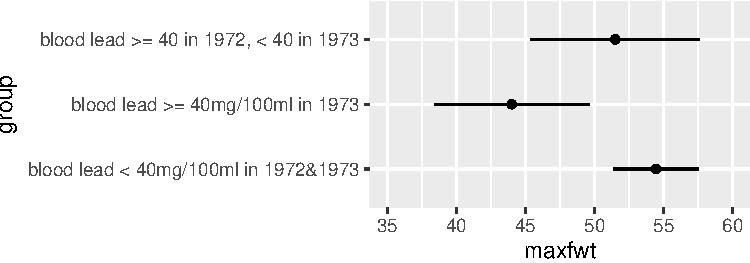
\includegraphics[width=\maxwidth]{reg-olslead-1} }


\begin{Schunk}
\begin{Sinput}
options(prType='plain')
summary(f)
\end{Sinput}
\begin{Soutput}
             Effects              Response : maxfwt 

 Factor                                                                             
 group - blood lead >= 40mg/100ml in 1973:blood lead < 40mg/100ml in 1972&1973      
 group - blood lead >= 40 in 1972, < 40 in 1973:blood lead < 40mg/100ml in 1972&1973
 Low High Diff. Effect   S.E.   Lower 0.95 Upper 0.95
 1   2    NA    -10.4380 3.2168 -16.8230   -4.0522   
 1   3    NA     -2.9375 3.4415  -9.7688    3.8938   
\end{Soutput}
\begin{Sinput}
options(prType='latex')
\end{Sinput}
\end{Schunk}
\bi
\item In general requires $k-1$ dummies to describe $k$ categories
\item For testing or prediction, choice of reference cell is
  irrelevant
\item Does matter for interpreting individual coefficients
\item Modern statistical programs automatically generate indicator
  variables from categorical or character predictors\footnote{In
    \R\ indicators are generated automatically any time a \Co{factor}
    or \Co{category} variable is in the model.}
\item In \R\ never generate indicator variables yourself; just provide a \co{factor} or \co{character} predictor.
\ei
\clearpage

\subsection{Obtaining ANOVA with Multiple Regression}\sound{reg-17}
\bi
\item Estimate $\alpha, \beta_{j}$ using standard least squares
\item $F$-test for overall regression is exactly $F$ for ANOVA
\item In ANOVA, $SSR$ is call sum of squares between treatments
\item $SSE$ is called sum of squares within treatments
\item Don't need to learn formulas specifically for ANOVA
\ei

\subsection{One-Way Analysis of Covariance} \ros{12.5.3}
\bi
\item Just add other variables (covariates) to the model
\item Example: predictors age and treatment \\
  age is the covariate (adjustment variable)
\item Global $F$ test tests the global null hypothesis that neither
  age nor treatment is associated with response
\item To test the adjusted treatment effect, use the partial $F$ test
  for treatment based on the partial $SS$ for treatment adjusted for
  age
\item If treatment has only two categories, the partial $t$-test is an
  easier way to get the age-adjusted treatment test
\begin{Sinput}
fa <- ols(maxfwt ~ age + group, data=lead)
fa
\end{Sinput}

 \centerline{\textbf{Linear Regression Model}}
 
 \begin{verbatim}
 ols(formula = maxfwt ~ age + group, data = lead)
 \end{verbatim}
 
 \begin{center}
 Frequencies of Missing Values Due to Each Variable
 
 \smallskip
 
 \begin{verbatim}
 maxfwt    age  group 
     25      0      0 
 \end{verbatim}
 
 \end{center}
 {\fontfamily{phv}\selectfont \begin{center}\begin{tabular}{|c|c|c|}\hline
&Model Likelihood&Discrimination\\
&Ratio Test&Indexes\\\hline
Obs~\hfill 99&LR $\chi^{2}$~\hfill 62.98&$R^{2}$~\hfill 0.471\\
$\sigma$~\hfill 9.4872&d.f.~\hfill 3&$R^{2}_{\textrm{adj}}$~\hfill 0.454\\
d.f.~\hfill 95&Pr$(>\chi^{2})$~\hfill 0.0000&$g$~\hfill 10.145\\
\hline
\end{tabular}
\end{center}}
 \begin{center}
 Residuals
 

 \begin{tabular}{ccccc}
Min&1Q&Median&3Q&Max\\
$-33.5$&$-5.125$&$0.9098$&$5.371$&$33$\\
\end{tabular}
 \end{center}
 
 %latex.default(U, file = "", first.hline.double = FALSE, table = FALSE,     longtable = TRUE, lines.page = lines.page, col.just = rep("r",         ncol(U)), rowlabel = "", already.math.col.names = TRUE,     append = TRUE)%
 \setlongtables\begin{longtable}{lrrrr}\hline
 \multicolumn{1}{l}{}&\multicolumn{1}{c}{$\hat{\beta}$}&\multicolumn{1}{c}{S.E.}&\multicolumn{1}{c}{$t$}&\multicolumn{1}{c}{Pr$(>|t|)$}\tabularnewline
 \hline
 \endhead
 \hline
 \endfoot
 Intercept&~27.2810~&~3.5303~& 7.73&\textless 0.0001\tabularnewline
 age&~ 2.6211~&~0.3209~& 8.17&\textless 0.0001\tabularnewline
 group=blood lead $\geq$ 40mg/100ml in 1973&~-7.5148~&~2.5043~&-3.00&0.0034\tabularnewline
 group=blood lead $\geq$ 40 in 1972, $\textless $ 40 in 1973&~-1.7464~&~2.6557~&-0.66&0.5124\tabularnewline
 \hline
 \end{longtable}
 \addtocounter{table}{-1}
\begin{Sinput}
ggplot(Predict(fa, age, group))
\end{Sinput}


\centerline{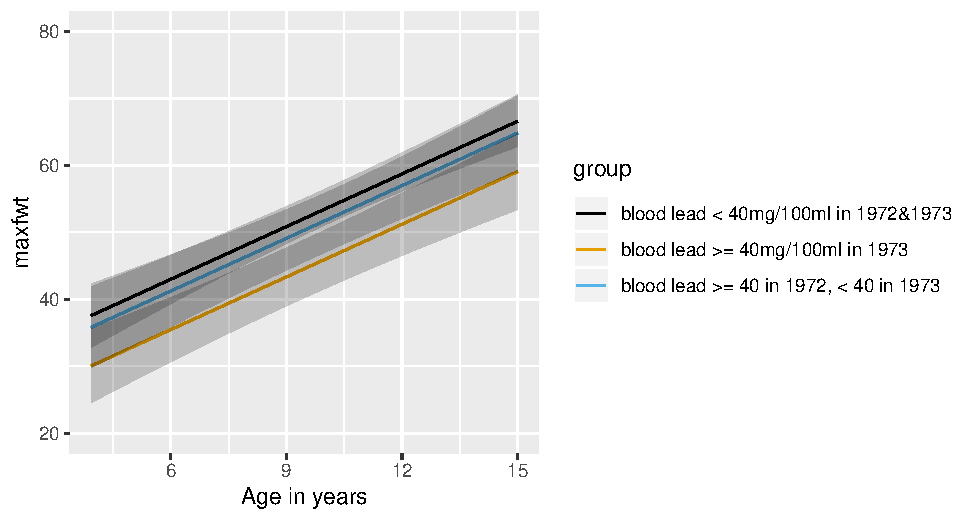
\includegraphics[width=\maxwidth]{reg-leadgrage-1} }


\begin{Schunk}
\begin{Sinput}
options(prType='plain')
summary(fa)
\end{Sinput}
\begin{Soutput}
             Effects              Response : maxfwt 

 Factor                                                                             
 age                                                                                
 group - blood lead >= 40mg/100ml in 1973:blood lead < 40mg/100ml in 1972&1973      
 group - blood lead >= 40 in 1972, < 40 in 1973:blood lead < 40mg/100ml in 1972&1973
 Low    High   Diff.  Effect  S.E.   Lower 0.95 Upper 0.95
 6.1667 12.021 5.8542 15.3440 1.8789  11.6140   19.0740   
 1.0000  2.000     NA -7.5148 2.5043 -12.4860   -2.5431   
 1.0000  3.000     NA -1.7464 2.6557  -7.0187    3.5259   
\end{Soutput}
\begin{Sinput}
options(prType='latex')
\end{Sinput}
\end{Schunk}
\begin{Sinput}
anova(fa)
\end{Sinput}
%latex.default(dstats, title = title, caption = if (table.env) caption else NULL,     insert.top = if (length(caption) && !table.env) paste0("\\Needspace{2in}\n",         caption), rowlabel = "", col.just = rep("r", length(sn)),     table.env = table.env, ...)%
\textbf{\Needspace{2in}
Analysis of Variance for \texttt{\smaller maxfwt}}\begin{center}
\begin{tabular}{lrrrrr}
\hline\hline
\multicolumn{1}{l}{}&\multicolumn{1}{c}{d.f.}&\multicolumn{1}{c}{Partial SS}&\multicolumn{1}{c}{MS}&\multicolumn{1}{c}{$F$}&\multicolumn{1}{c}{$P$}\tabularnewline
\hline
age& 1&6003.1719&6003.17189&66.70&\textless 0.0001\tabularnewline
group& 2& 810.4561& 405.22806& 4.50&0.0135\tabularnewline
\textbf{REGRESSION}& 3&7603.2603&2534.42009&28.16&\textless 0.0001\tabularnewline
\textbf{ERROR}&95&8550.5781&  90.00609&&\tabularnewline
\hline
\end{tabular}\end{center}
\begin{Sinput}
anova(f)    # reduced model (without age)
\end{Sinput}
%latex.default(dstats, title = title, caption = if (table.env) caption else NULL,     insert.top = if (length(caption) && !table.env) paste0("\\Needspace{2in}\n",         caption), rowlabel = "", col.just = rep("r", length(sn)),     table.env = table.env, ...)%
\textbf{\Needspace{2in}
Analysis of Variance for \texttt{\smaller maxfwt}}\begin{center}
\begin{tabular}{lrrrrr}
\hline\hline
\multicolumn{1}{l}{}&\multicolumn{1}{c}{d.f.}&\multicolumn{1}{c}{Partial SS}&\multicolumn{1}{c}{MS}&\multicolumn{1}{c}{$F$}&\multicolumn{1}{c}{$P$}\tabularnewline
\hline
group& 2& 1600.088&800.0442&5.28&0.0067\tabularnewline
\textbf{REGRESSION}& 2& 1600.088&800.0442&5.28&0.0067\tabularnewline
\textbf{ERROR}&96&14553.750&151.6016&&\tabularnewline
\hline
\end{tabular}\end{center}

Subtract SSR or SSE from these two models to get the treatment effect with 2 d.f.
\ei

\subsection{Continuous Analysis of Lead Exposure}
See \ref{sec:rmsintro-leadcontinuous}.

\subsection{Two-Way ANOVA} \ros{12.6}\sound{reg-18}
\bi
\item Two categorical variables as predictors
\item Each variable is expanded into indicator variables
\item One of the predictor variables may not be time or episode within
  subject; two-way ANOVA is often misused for analyzing repeated
  measurements within subject
\item Example: 3 diet groups (NOR, SV, LV) and 2 sex groups
\item $E(y|diet,sex) = \alpha + \beta_{1}[SV] + \beta_{2}[LV] +
  \beta_{3}[male]$
\item Assumes effects of diet and sex are additive (separable) and not
  synergistic
\item $\beta_{1} = SV - NOR$ mean difference holding sex constant \\
  $\beta_{3} = male - female$ effect holding diet constant
\item Test of diet effect controlling for sex effect: \\
 $H_{0}:\beta_{1}=\beta_{2}=0$ \\
 $H_{a}: \beta_{1} \neq 0$ or $\beta_{2} \neq 0$
\item This is a 2 d.f.\ partial $F$-test, best obtained by taking
  difference in $SS$ between this full model and a model that excludes
  all diet terms.
\item Test for significant difference in mean $y$ for males vs.\
  females, controlling for diet: \\
 $H_{0}: \beta_{3} = 0$
\item For a model that has $m$ categorical predictors (only), none of
  which interact, with numbers of categories given by $k_{1}, k_{2},
  \ldots, k_{m}$, the total numerator regression d.f.\ is
  $\sum_{i=1}^{m}(k_{i}-1)$
\ei

\subsection{Two-way ANOVA and Interaction}
\disc{reg-ia}
Example: sex (F,M) and treatment (A,B) \\
Reference cells: F, A\\

Model: \\
\beqa
E(y|sex,treatment) &=& \alpha + \beta_{1}[sex=M] \\
 &+& \beta_{2}[treatment=B] + \beta_{3}[sex=M \cap treatment=B]
\eeqa
Note that $[sex=M \cap treatment=B] = [sex=M] \times
[treatment=B]$.
\begin{description}
\item[$\alpha$]: mean $y$ for female on treatment A (all variables at
  reference values)
\item[$\beta_{1}$]: mean $y$ for males minus mean for females, both on
  treatment $A$ = sex effect holding treatment constant at $A$
\item[$\beta_{2}$]: mean for female subjects on treatment $B$ minus
  mean for females on treatment $A$ = treatment effect holding sex
  constant at $female$
\item[$\beta_{3}$]: $B-A$ treatment difference for males minus $B-A$
  treatment difference for females \\
 Same as $M-F$ difference for treatment $B$ minus $M-F$ difference for
 treatment $A$
\end{description}
In this setting think of interaction as a ``double difference''.  To
understand the parameters:
\ipacue\btable{ll}{}\hline
Group & $E(y|Group)$ \\ \hline
F~A & $\alpha$ \\
M~A & $\alpha + \beta_{1}$ \\
F~B & $\alpha + \beta_{2}$ \\
M~B & $\alpha + \beta_{1} + \beta_{2} + \beta_{3}$ \\ \hline
\etable
Thus $MB - MA - [FB - FA] = \beta_{2} + \beta_{3} - \beta_{2} =
\beta_{3}$.

\subsubsection{Heterogeneity of Treatment Effect}\sound{reg-19}\disc{reg-hte}
Consider a Cox proportional hazards model for time
until first major cardiovascular event.  The application is targeted
pharmacogenomics in acute coronary syndrome (the CURE study~\cite{par10eff}).

\bi
\item Subgroup analysis is virtually worthless for learning about
  differential treatment effects
\item Instead a proper assessment of interaction must be used, with
  liberal adjustment for main effects
\item An interaction effect is a double difference; for logistic and
  Cox models it is the ratio of ratios
\item Interactions are harder to assess than main effects (wider
  confidence intervals, lower power)
\item Carriers for loss-of-function CYP2C19 alleles:\ipacue
reduced conversion of clopidogrel to active metabolite
\item Suggested that clop.\ less effective in reducing CV death, MI,
stroke
\item 12,562 (clop.\ HR 0.8); 5059 genotyped (clop.\ HR 0.7)
\ei

\begin{center}\begin{tabular}{lccc} \hline
& Carrier & & Non-Carrier\\ \hline
HR & 0.69 {\smaller (0.49, 0.98)} & & 0.72 {\smaller (0.59, 0.87)} \\ \hline
Ratio & & 0.96 {\smaller (0.64, 1.43)} & \\
of HRs & & {\smaller ($P=0.8$)} & \\ \hline
\end{tabular}\end{center}

\bi
\item In the publication the needed ratio of hazard ratios was nowhere
  to be found
\item C.L.\ for ratio of hazard ratios shows that CYP2C19 variants may
  plausibly be associated with a huge benefit or huge harm
\item Point estimate is in the wrong direction
\item Epidemiologic evidence points to a dominant effect of smoking in
  this setting
 \bi
  \item Significant interaction between smoking status and clop.\ effect
  \item Lack of evidence that clop.\ is effective in non-smokers
  \item Gurbel, Nolin, Tantry, JAMA 2012:307:2495
 \ei
\ei
%http://jama.jamanetwork.com/article.aspx?articleID=1187938&utm_source=Silverchair%20Information%20Systems&utm_medium=email&utm_campaign=MASTER%3A_JAMA_Latest_Issue_TOC_Notification_06%2F20%2F2012


\subsection{Interaction Between Categorical and Continuous Variables}%
\sound{reg-20} \disc{reg-ia-cc}
This is how one allows the slope of a predictor to vary by categories
of another variable.  Example: separate slope for males and females:
\beqa
E(y|x) &=& \alpha + \beta_{1}age + \beta_{2}[sex=m] \\
       &+& \beta_{3}age\times [sex=m] \\
E(y|age, sex=f) &=& \alpha + \beta_{1}age \\
E(y|age, sex=m) &=& \alpha + \beta_{1}age + \beta_{2} + \beta_{3}age \\
                &=& (\alpha + \beta_{2}) + (\beta_{1}+\beta_{3})age
\eeqa
\bd
\item[$\alpha$]: mean $y$ for zero year-old female
\item[$\beta_{1}$]: slope of age for females
\item[$\beta_{2}$]: mean $y$ for males minus mean $y$ for females, for
  zero year-olds
\item[$\beta_{3}$]: increment in slope in going from females to males
\ed

\section{Internal vs.\ External Model Validation}\sound{reg-21}
\disc{reg-val}\label{reg-val}
\blog{split-val}
\quoteit{External validation or validation on a holdout sample, when
  the predictive method was developed using feature selection, model
  selection, or machine learning, produces a non-unique \emph{example}
  validation of a non-unique \emph{example} model.}{FE Harrell, 2015}

\bi
\item Many researchers assume that ``external'' validation of model
  predictions is the only way to have confidence in predictions
\item External validation may take years and may be low precision
  (wide confidence intervals for accuracy estimates)
\item Splitting one data sequence to create a holdout sample is
  \emph{internal} validation, not \emph{external}, and resampling
  procedures using all available data are almost always better
\item External validation by splitting in time or place loses
  opportunity for modeling secular and geographic trends, and often
  results in failure to validate when in fact there are interesting
  group differences or time trends that could have easily been modeled
\item One should use all data available at analysis time\ipacue
\item External validation is left for newly collected data not
  available at publication time
\item Rigorous internal validation should be done first
  \bi
  \item ``optimism'' bootstrap generally has lowest mean squared error
    of accuracy estimates
  \item boostrap estimates the likely future performance of model
    developed on whole dataset
  \item all analytical steps using $Y$ must be repeated for each of
    approx.\ 300-400 bootstrap repetitions
  \item when empirical feature selection is part of the process, the bootstrap
    reveals the true volatility in the list of selected predictors
  \ei
\item Many data splitting or external validations are unreliable \ipacue
  (example: volatility of splitting 17,000 ICU patients with high
  mortality, resulting in multiple splits giving different models and
  different performance in holdout samples)
\ei

There are subtleties in what holdout sample validation actually means,
depending on how he predictive model is fitted:
\bi
\item When the model's form is fully pre-specified, the external
  validation validates that model and its estimated coefficients
\item When the model is derived using feature selection or machine
  learning methods, the holdout sample validation is not ``honest'' in
  a certain sense:
  \bi
  \item data are incapable of informing the researcher what the
    ``right'' predictors and the ``right'' model are
  \item the process doesn't recognize that the model being validated
    is nothing more than an ``example'' model
  \ei
\item Resampling for rigorous internal validation validates the\ipacue
  \emph{process} used to derive the ``final'' model
  \bi
  \item as a byproduct estimates the likely future performance of that model
  \item while reporting volatility instead of hiding it
  \ei
\ei

Model validation is a very important and complex topic that is covered
in detail in the two books mentioned below.  One of the most
difficult to understand elements of validation is what is, and when to
use, external validation.  Some researchers have published predictive
tools with no validation at all while other researchers falsely
believe that ``external'' validation is the only valid approach to
having confidence in predictions.  Frank Harrell (author of
\emph{Regression Modeling Strategies}) and Ewout Steyerberg
(author of \emph{Clinical Prediction Models})
have written the text below in an attempt to illuminate several issues.

{\smaller
There is much controversy about the need for, definition of, and
timing of external validation.
A prognostic model should be valid outside the specifics of the sample
where the model is developed. Ideally, a model is shown to predict
accurately across a wide range of settings (Justice et al, \emph{Ann Int
		Med} 1999).  Evidence of such external validity requires evaluation by
different research groups and may take several years.  Researchers
frequently make the mistake of labeling data splitting from a single
sequence of patients as external validation when in fact this is a
particularly low-precision form of internal validation better done
using resampling (see below).  On the other hand, external validation
carried out by by splitting in time (temporal validation) or by place,
is better replaced by considering interactions in the full dataset.  For
example, if a model developed on Canadians is found to be poorly
calibrated for Germans, it is far better to develop an international
model with country as one of the predictors.  This implies that a
researcher with access to data is always better off to analyze and
publish a model developed on the full set.  That leaves external
validation using (1) newly collected data, not available at the time
of development; and (2) other investigators, at other sites, having
access to other data. (2) has been promoted by Justice as the
strongest form of external validation.  This phase is only relevant
once internal validity has been shown for the developed model.  But
again, if such data were available at analysis time, those data are
too valuable not to use in model development.

Even in the small subset of studies comprising truly external
validations, it is a common misconception that the validation statistics
are precise.  Many if not most external validations are unreliable due to
instability in the estimate of predictive accuracy.  This instability
comes from two sources: the size of the validation sample, and the
constitution of the validation sample.  The former is easy to
envision, while the latter is more subtle.  In one example, Frank
Harrell analyzed 17,000 ICU patients with $\frac{1}{3}$ of patients dying,
splitting the dataset into two halves - a training sample and a
validation sample.  He found that the validation c-index (ROC area)
changed substantially when the 17,000 patients were re-allocated at
random into a new training and test sample and the entire process
repeated.  Thus it can take quite a large external sample to yield
reliable estimates and to "beat" strong internal validation using
resampling.  Thus we feel there is great utility in using strong
internal validation.

At the time of model development, researchers should focus on showing
internal validity of the model they propose, i.e. validity of the
model for the setting that they consider.  Estimates of model
performance are usually optimistic. The optimism can efficiently be
quantified by a resampling procedure called the bootstrap, and the
optimism can be subtracted out to obtain an unbiased estimate of
future performance of the model on the same types of patients.  The
bootstrap, which enjoys a strong reputation in data analysis, entails
drawing patients from the development sample with replacement.  It
allows one to estimate the likely future performance of a predictive
model without waiting for new data to perform a external validation
study.  It is important that the bootstrap model validation be done
rigorously. This means that all analytical steps that use the outcome
variable are repeated in each bootstrap sample.  In this way, the
proper price is paid for any statistical assessments to determine the
final model, such as choosing variables and estimating regression
coefficients.  When the resampling allows models and coefficients to
disagree with themselves over hundreds of resamples, the proper price
is paid for "data dredging", so that clinical utility (useful
predictive discrimination) is not claimed for what is in fact
overfitting (fitting "noise").  The bootstrap makes optimal use of the
available data: it uses all data to develop the model and all data to
internally validate the model, detecting any overfitting.  One can
call properly penalized bootstrapping rigorous or strong internal
validation.
}

To properly design or interpret a predictive model validation it is
important to take into account how the predictions were formed.  There
are two overall classes of predictive approaches:
\bi
\item formulating a pre-specified statistical model based on
  understanding of the literature and subject matter and using the
  data to fit the parameters of the model but not to select the
  \emph{form} of the model or the features to use as predictors
\item using the data to screen candidate predictive features or to
  choose the form the predictions take.  Examples of this class
  include univariable feature screening, stepwise regression, and
  machine learning algorithms.
\ei
External holdout sample validation may seem to be appropriate for the
second class but actually it is not ``honest'' in the following
sense.  The data are incapable of informing the researcher of what are
the ``right'' predictors.  This is even more true when candidate
predictors are correlated, creating competition among predictors and
arbitrary selections from these co-linear candidates.  A predictive
rule derived from the second class of approaches is merely an
\emph{example} of a predictive model.  The only way for an analyst to
understand this point is to use resampling (bootstrap or
cross-validation) whereby predictive models (or machine learning
structures) are repeatedly derived from scratch and the volatility (and
difficulty of the task) are exposed.

So what goes in in the training and validation processes depends on
the class of predictive methods used:
\bi
\item When the model is pre-specified except for the regression
  coefficients that need to be estimated, rigorous resampling
  validation validates the fit of \emph{the} model and so does holdout
  sample validation.
\item When the model structure was not pre-specified but model/feature
  selection was done, resampling validation validates the
  \emph{process} used to derive the ``final'' model and as a
  by-product estimates the likely future performance of this model
  while documenting to the researcher that there is usually great
  instability in the form of this model.  It is imperative that the
  analyst repeat \emph{all} feature selection or model selection steps
  afresh for each resample and displays the variation of features /
  models selected across the resamples.  For the bootstrap this
  usually involves 300 or more resamples, and for cross-validation 50
  or more repeats of 10-fold cross-validation.  The ``final'' model
  should be describe as an example of an entire array of models, and
  the likely future performance of this example model is estimated
  from the resampling procedure just described.  Resampling alerts the
  analyst alert to arbitrariness and reduces the tendency to cherry
  pick good validations when split-sample or external validation is used.
\ei

Thus in the case just described where a statistical model is not fully
pre-specified, pretending to ``freeze'' the ``final'' result and
validating it on a holdout sample is problematic.  The resulting
validation, far from being a validation of ``the'' model is just an
example validation of an example model.  On the other hand, rigorous
validation using resampling validates the process used to derive the
final predictive instrument, while still providing a good estimate of
the likely future predictive accuracy of that instrument.

\subsection{Summary: Choosing Internal vs.\ External Validation}\label{reg-choose-val}
Recall that strong internal validation uses the bootstrap in a way
that repeats all modeling steps (feature/variable selection, transformation
selection, parameter estimation, etc.) that utilized the outcome
variable $Y$.

Use strong internal validation if
\bi
\item the model is not pre-specified.  If any feature selection
  utilizing $Y$ was done, the set of features selected will be
  unstable, so an external validation would just validate an ``example
  model.''  On the other hand, a strong internal validation validates
  the model development \emph{process} and fully documents the
  volatility of feature selection.
\item the data come from multiple locations or times and you want to
  understand time trends in $Y$, or geographic differences
\item the size of the potential external validation sample and the
  size of the training sample are not both very large
\ei

Use external validation if
\bi
\item measurement platforms vary (e.g., genotyping or blood analysis
  equipment) and you want to validate the generalizability of a model
  developed on your platform
\item both the training data and the test datasets are very large
  (e.g., the training data contains more than 15 events per
  \textbf{candidate} predictor and the test data has at least 200-400 events)
\item the dataset to be used for the external validation was not
  available when the model was developed and internally validated
\item you don't trust the model developers to honestly perform a
  strong internal validation
\ei

\subsection{Other Resources}
\bi
\item
  \href{http://www.cecilejanssens.org/wp-content/uploads/2018/01/PredictionManual2.0.pdf}{Prediction Research Manual} by Cecile Janssens and Forike Martens
  \item Steyerberg paper on the waste by data splitting~\cite{ste18vala}.
\ei

\def\apacue{0}
